% mnras_template.tex 
%
% LaTeX template for creating an MNRAS paper
%
% v3.0 released 14 May 2015
% (version numbers match those of mnras.cls)
%
% Copyright (C) Royal Astronomical Society 2015
% Authors:
% Keith T. Smith (Royal Astronomical Society)

% Change log
%
% v3.0 May 2015
%    Renamed to match the new package name
%    Version number matches mnras.cls
%    A few minor tweaks to wording
% v1.0 September 2013
%    Beta testing only - never publicly released
%    First version: a simple (ish) template for creating an MNRAS paper

%%%%%%%%%%%%%%%%%%%%%%%%%%%%%%%%%%%%%%%%%%%%%%%%%%
% Basic setup. Most papers should leave these options alone.
\documentclass[fleqn,usenatbib]{mnras}

% MNRAS is set in Times font. If you don't have this installed (most LaTeX
% installations will be fine) or prefer the old Computer Modern fonts, comment
% out the following line
\usepackage{newtxtext,newtxmath}
% Depending on your LaTeX fonts installation, you might get better results with one of these:
%\usepackage{mathptmx}
%\usepackage{txfonts}

% Use vector fonts, so it zooms properly in on-screen viewing software
% Don't change these lines unless you know what you are doing
\usepackage[T1]{fontenc}
\usepackage{float}

% Allow "Thomas van Noord" and "Simon de Laguarde" and alike to be sorted by "N" and "L" etc. in the bibliography.
% Write the name in the bibliography as "\VAN{Noord}{Van}{van} Noord, Thomas"
\DeclareRobustCommand{\VAN}[3]{#2}
\let\VANthebibliography\thebibliography
\def\thebibliography{\DeclareRobustCommand{\VAN}[3]{##3}\VANthebibliography}


%%%%% AUTHORS - PLACE YOUR OWN PACKAGES HERE %%%%%

% Only include extra packages if you really need them. Common packages are:
\usepackage{graphicx}	% Including figure files
\usepackage{amsmath}	% Advanced maths commands
% \usepackage{amssymb}	% Extra maths symbols
\usepackage{subfigure}
\usepackage{siunitx}
%%%%%%%%%%%%%%%%%%%%%%%%%%%%%%%%%%%%%%%%%%%%%%%%%%

%%%%% AUTHORS - PLACE YOUR OWN COMMANDS HERE %%%%%

% Please keep new commands to a minimum, and use \newcommand not \def to avoid
% overwriting existing commands. Example:
%\newcommand{\pcm}{\,cm$^{-2}$}	% per cm-squared

%%%%%%%%%%%%%%%%%%%%%%%%%%%%%%%%%%%%%%%%%%%%%%%%%%

%%%%%%%%%%%%%%%%%%% TITLE PAGE %%%%%%%%%%%%%%%%%%%

% Title of the paper, and the short title which is used in the headers.
% Keep the title short and informative.
\title[Short title, max. 45 characters]{Measuring the evolution of early-type galaxies in GAMA using observationally robust  quantities}

% The list of authors, and the short list which is used in the headers.
% If you need two or more lines of authors, add an extra line using \newauthor
\author[Rongfu Liu et al.]{
Rongfu Liu, Alessandro Sonnenfeld
% List of institutions
}

% These dates will be filled out by the publisher
\date{Accepted XXX. Received YYY; in original form ZZZ}

% Enter the current year, for the copyright statements etc.
\pubyear{2023}

% Don't change these lines
\begin{document}
\label{firstpage}
\pagerange{\pageref{firstpage}--\pageref{lastpage}}
\maketitle

% Abstract of the paper
\begin{abstract}
test This is a simple template for authors to write new MNRAS papers.
The abstract should briefly describe the aims, methods, and main results of the paper.
It should be a single paragraph not more than 250 words (200 words for Letters).
No references should appear in the abstract.
\end{abstract}

% Select between one and six entries from the list of approved keywords.
% Don't make up new ones.
\begin{keywords}
keyword1 -- keyword2 -- keyword3
\end{keywords}

%%%%%%%%%%%%%%%%%%%%%%%%%%%%%%%%%%%%%%%%%%%%%%%%%%

%%%%%%%%%%%%%%%%% BODY OF PAPER %%%%%%%%%%%%%%%%%%

\section{Introduction}
% \cite{van_dokkum_1996}
\par Early type galaxies (ETGs) ,which are typically elliptical in shape, are believed to be passively evolved after their star-forming activities being quenched. Over the past few decades, observations have confirmed that the ETGs at the epoch of $z \approx 2 $ are much more compact than their counterpart at $z \approx 0$ (\cite{daddiPassivelyEvolvingEarlyType2005}, \cite{toft2007}, \cite{trujillo2006}, \cite{trujillo2007}, \cite{vandokkum2008}). These ultra-compact objects then experienced a dramatic growth in size, in particular, by about a factor of 3 between $z = 2 $ and $ z = 0$( \cite{damjanov2019, fan_dramatic_2008, hamadouche2022, vanderwel3DHSTCANDELSEvolution2014, van_dokkum_growth_2010}). 
% have a more significant growth in size comparing to their star-forming counterpart.
% Currently, the most popular formation scenario of ETGs consists of two phases. At early time ($z > 2$), proto-ellipticals are formed in an intense star-forming activities with strong gas dissipation process which drive these galaxies to be extremely compact. Most of the stellar mass of such systems are gained through this first phase of formation. While in the second phase, it is well agreed that the growth was dominated by minor mergers, resulting in a "puffing-up" in size and a moderate growth in stellar mass.
Numerous  works in literature have confirmed that the dissipationless dry mergers is the major mechanism that attribute to that rapid size growth. 
(e.g.  \cite{naab_minor_2009},\cite{van_dokkum_2010_hubble}, \cite{oser_cosmological_2011},\cite{newman2012},  \cite{hilz_how_2013}, \cite{dekel_wet_2014}, \cite{deugenio2023}), especially for mergers with mass ratio around 1:10(\cite{newman2012,Belli_2015}). However, purely minor merger is not sufficient to explain the entire growth , or the number of mergers will be too large in that case(\cite{hopkins_discriminating_2010,nipoti2009}) while the constrain placed by the density slope of galaxies cannot be satisfied (\cite{sonnenfeld2014}). Some other mechanisms or observational effects must be taken into consideration, such as dry mergers with higher mass ratio (major merger) and the existence of the color gradient. 
% Nevertheless, the mechanism that lead to such "puffing-up" are still undetermined. Both non-dissipating dry mergers(\cite{van_dokkum_2010_hubble})and quasar feedback (\cite{fan_dramatic_2008}) can be a reasonable explanation .in addition with some secondary effects, ,
\par At relatively lower redshift, newly queched galaxies may join the population of quiescent galaxies. These "fresh blood" of quiescent population are relatively larger, thus could mimic the growth in size of such galaxies.This effect is called "progenitor bias"(\cite{van_dokkum_1996,carolloNEWLYQUENCHEDGALAXIES2013, fagioliMinorMergersProgenitor2016, vandokkumMorphologicalEvolutionAges2001}), and it is also an important effect that may contribute to the observed size evolution of ETGs. Each of these effect will leave impact on some other observable properties of galaxy, such as velocity dispersion, number density and mass, while these impact could in turn place constrains on the effects above. Nevertheless, a theoretical model that could meet all these constrains is still in absence.   
\par Besides, another systematic might be ignored in the literature.The problem arise from the finite photometric depth of observations. it is hard to measure the total light directly (\cite{tal_2011_faint}) as the information where the surface brightness of galaxies drops below the observation limit remains unknown. To obtain a accurate measurement of the total light, a precise sky-subtraction is demanded while it is easy to bring additional systematic. In literature, we use various models to fit the surface brightness distribution of galaxies . The faint outskirt of galaxies could not provide reliable constrains during the fitting process, thus the model could not be able to provide reliable descriptions for surface brightness there . These unreliable data will be accounted in the total light measurement and will take up an ineligible fraction(up to 20\% according to \cite{Alessandro20}).However, the traditional definition of galaxy size and mass derived from the best-fit model are both associated with the total light, therefore we believe they are not robust qualities. 
% Both half-light radius and total stellar mass that derived from the best-fit model are associated with total light , and thus we believe that the traditional definition of galaxy size and mass is not robust. 
\par Instead of investigating the whole galaxy, we may focus on a fixed, relatively small aperture and investigate some properties inside, following the method proposed in \cite{Alessandro20}. In this work, we choose 10kpc as that aperture,in consideration that it is large enough to enclose sufficient amount of stellar mass while will not be too large to suffer from the extrapolation problem. We use $M_{*,10}$ to denote the mass enclosed inside 10kpc and $\Gamma_{*,10}$ to represent to mass-weighted projected surface density slope.The latter is defined as
\begin{equation}
    \Gamma_{*,10} = \frac{2\pi \int_0^{10} R \frac{dlog\Sigma_*}{dlogR}\Sigma_*(R)dR}{2\pi \int_0^{10}R\Sigma_*(R)dR} = 2 - \frac{2\pi \times 10^2 \times \Sigma_*(10)}{M_{*,10}}
\end{equation} 
% \par In context of merger, the growth in size of one single galaxies can be approximated by Virial Theorem, assuming a isothermal density profile( \cite{naab_minor_2009}).
\par Assuming a isothermal density profile for elliptical galaxy, the growth in total stellar mass and effective radius due to mergers can be approximated using virial theorem\citep{naab_minor_2009}. In particular, if the mass of one galaxy grow by a factor of $\eta$, i.e. $M_f = (1+\eta) M_i$, then the growth of gravititional radius can be expressed as $r_f = \frac{(1+\eta)^2}{(1+\eta \epsilon)} r_i$ , here $\epsilon$ is the ratio of mean square velocity of the accreted galaxy to that of the progenitor galaxy.
%  we can obtain a strict relation between $\Delta M_*$ and $\Delta R_e$ depending on different merger scenarios
 . However, switching to $M_{*,10}$ and $\Gamma_{*,10}$ space, it's hard to derive a relation in $\Delta M_{*,10}$ and $\Delta \Gamma_{*,10}$ analytically as a fixed aperture size 10kpc is involved. Nevertheless, N-body simulations can be helpful. We utilize the simulation result from \cite{nipoti2009} which contains a number of binary mergers with different mass ratio. We measure the $M_{*,10}$ and $\Gamma_{*,10}$ of both progenitor and merger remnant and calculate the growth in these two quantities. In addition to finding that different merger ratio behaves differently, we also discovered that the scale of galaxy also make diferences. 
\par Having find how the $M_{*,10}$ and $\Gamma_{*,10}$ under different growth scenarios, we then compared them with the evolution of these two quantities in reality. We select ETGs from GAMA DR4 main survey (Galaxy and Mass Assembly, \cite{GAMAmain};\cite{bellstedt_galaxy_2020} ; \cite{GAMA1}; \cite{GAMA2}) and obtained precise spectroscopic redshift and other quantities that related to spectrum measurement, e.g. stellar mass. In addition, 
% we use the 2DPHOT structural parameter catalogue from KiDs DR4 
the structural parameter are measured from KiDs photometry (Kile Degree survey , \cite{kuijken_fourth_2019}, \cite{KiDs_Roy}, \cite{Amaro_rejection_2021}) using GalNet (\cite{GaLNet2022}). Based on these observation datas,  we then calculated their $M_{*,10} $ and $\Gamma_{*,10}$ and further analyse the , $M_{*,10} - \Gamma_{*,10}$ relation and their evolution from $z = 0.6$ to present. 
% * focus inside 10kpc
% \par By focusing inside $10kpc$, we are automatically able to know if and how the stellar mass of inner region grow. In the context of two-phase formation scenario of ETGs, during the second evolution phase, the total stellar mass will grow insignificantly, and is confirmed by observations recently (\cite{Bundy2017}) . In contrast, due to the undetermined mechanism that drive galaxy to extend, we are still not clear the behaviour of inner region through the second phase. In literature, \cite{van_dokkum_growth_2010} stacked the images of numerous galaxies and found the mass show no signal to grow in inner 5 kpc  of ETGs. Recently , take the advantage of the development of Integral Field Spectroscopy(IFS), several studies have been trying to recover the evolution histories using local, spatially resolved galaxies (cite). 

% Although our resolution is not comparable to MANGAs, our sample choice can extend to higher redshift with larger sample amount. While in comparison with \cite{van_dokkum_growth_2010}, we have better images, thus don't need to stack all the images. 
% \par Using $M_{*,10}$ along, we are able to study the evolution of inner region of galaxies.  Combining with $\Gamma_{*,10}$, we have a robust set of parameters to describe the mass density profile of galaxies. $\Gamma_{*,10} $ is, by definition, the average slope of the surface density profile inside 10 $kpc$, thus encode the information about how compact one galaxy is. Actually, the combination of $M_{*,10}$ and $\Gamma_{*,10}$ can provide a precise description of surface density slope in inner $10  kpc $ better than 20\% \cite{Alessandro20}. We believe it is reasonable to measure the growth in size of ETGs using this parameterization.  
% using this set of parameters, we are able to measure the evolution in density profile of ETGs and might indicate how the size of galaxies grow.   
% \par In this work, we select ETGs from GAMA DR4 main survey (Galaxy and Mass Assembly, \cite{GAMAmain};\cite{bellstedt_galaxy_2020} ; \cite{GAMA1}; \cite{GAMA2}) and obtained most of the qutities we want, such as total stellar mass, redshift etc.. In addition, we use the 2DPHOT structural parameter catalogue from KiDs DR4 ( Kile Degree survey , \cite{kuijken_fourth_2019}, \cite{KiDs_Roy}, \cite{Amaro_rejection_2021}) to give most of ETGs reasonable sersic parameters in complement. For the rest galaxies, we use GALFIT (\cite{Peng_galfit_2002}, \cite{Peng_galfit_2010}) to operate a single sersic fitting to obtain their sersic parameters. Then we calculate their $M_{*,10} $ and $\Gamma_{*,10}$ and further analyse the $M_{*,10} $ funtion, $M_{*,10} - \Gamma_{*,10}$ funtion and their evolution from $z = 0.6$ to present. 
\par The structure of this paper is as follows. In Sect.\ref{sec:2}, we give a brief description on both observations from KiDs\&GAMA and the binary merger simulation from \citep{nipoti2009}. I present the result of growth of $M_{*,10}$ and $M_{*,10}-\Gamma_{*,10}$ in different merger scenarios in Sect.3  and present the comparison with observation result in Sect.4. Finally, I give a discussion in Sect.5 then conclude the paper in Sect.6.
\par In this paper, we assume a flat $\Lambda$CDM cosmology with $\Omega_M = 0.3$ and $H_0 = 70 km ~s^{-1}~Mpc^{-1}$. Magnitude are in AB units and stellar mass are in solar units.
% In fact, $\Gamma_{*,10}$ tells us how compact one galaxy are, thus could be a reasonable indicator of the galaxy size instead of the half-light radius $R_e$.Therefore, we can use a new set of parameter $M_{*,10}, \Gamma_{*,10}$ to investigate the evolution in mass and size of ETGs.Free from the extrapolation problem, our method might be able to provide a more robust measurement of the evolution in size of ETGs. 
% That is so called extrapolation problem.
% As is expected by existing theory, the mass and size of quiescent galaxies should evolve with time, and is confirmed by the observation result at the epoch of $z > 1$(some relating papers listed here).However, approaching a closer epoch ($z < 1$), the result becomes less conclusive. Various studies has focused on the evolution of the stellar mass function\citep{Bundy2017},the mass-velocity dispersion relation \citep{2020MNRAS.498.1101C} and the mass-size relation \citep{2019ApJ...872...91D}(to be refine). 
% \par These discrepancy may come from the measurement of stellar mass and the half-light radius. Traditionally, we fit the surface brightness of galaxies with some existing model(such as Sersic model) to infer its half-light radius and total stellar mass. However, this process might be biased by extrapolation problem \cite{Alessandro20} . In the outer region of galaxy, the brightness may drop below the background noise and thus introduce profound errors. To solve this problem, we adopt the method Alessandro suggested in his paper. Instead of investigating the whole galaxy, we may focus on a fixed, relatively small aperture and investigate some properties inside. In this paper, we'll choose 10kpc as the fixed aperture,which will be large enough to enclose sufficient amount of stellar mass while will not be too large to suffer from the extrapolation problem. We use $M_{*,10}$ to denote the mass enclosed inside 10kpc and $\Gamma_{*,10}$ to represent to mass-weighted projected surface brightness slope. In fact, $\Gamma_{*,10}$ tells us how compact one galaxy are, thus could be a reasonable indicator of the galaxy size instead of the half-light radius $R_e$.Therefore, we can use a new set of parameter $M_{*,10}, \Gamma_{*,10}$ to investigate the evolution in mass and size of ETGs.Free from the extrapolation problem, our method might be able to provide a more robust measurement of the evolution in size of ETGs. 
% \par In addition, these set of parameter automatically enable us to investigate whrere and how does the growth take place. \cite{Dokkum2010} invetigated this issue and found that the stellar mass inside 5kpc won't grow with time. The method he used is stacking the images of various galaxies, which is sensitive to sky subtraction and need to make some assumptions to galaxies, such as "all galaxies are identical". Up to now, we have better observations of ETGs, and it's not necessary to stack up the images. Therefore, we don't need the assumptions mentioned above and a free from the sensitivity of the sky subtraction, and we might be able to provide a more precise result about the grow in the region of one galaxy.   
% \par In this work, we choose the ETG sample from Galaxy And Mass Assembly survey (GAMA \cite{GAMAmain}; \cite{GAMA1}; \cite{GAMA2}) and use photometric data from Kilo-Degree survey(KiDs \cite{KiDs_Roy}). We measured the $M_{*,10}, \Gamma_{*,10}$ using the Sersic parameter provided by KiDs catalogue and plot the $M_{*,10}$ function at different redshift to investigate the mass growth in the inner region of ETGs. We further studied the $M_{*,10}-\Gamma_{*,10}$ relation and it's redshift-dependent evolution.We find blablabla ......
% \par The structure of this paper is as follows. In Sect.2, I described the spectroscopic and the photometric data from GAMA survey and KiDs survey respectively, and the method we use to ensure the completeness of sample. I present the result of growth of $M_{*,10}$ and $M_{*,10}-\Gamma_{*,10}$ relation in Sect.3  and discuss the result in Sect.4. Finally, I give a brief conclusion in Sect.6   
\section{Data}
\label{sec:2}
\subsection{observation sample selection}
\par In this work, we need precise redshift measurment to ensure the stellar mass and aperture size of 10 $kpc$ is accurate. Therefore, we choose to use more reliable spectroscopic redshift instead of photometric redshift, obtaining measurement from ETGs in GAMA DR4. 
% select early type galaxies from GAMA DR4, which could provide reliable spectroscopic redshift measurement.
In practice, I  use DMU gkvScienceCatv02(\cite{bellstedt_galaxy_2020}) to select galaxies from GAMA DR4 Main Survey sample, which only include galaxies whose r-band magnitude is larger than 19.65 in order to ensure the 95\% spec-z completeness of the sample. Further, I obtain the intensity of emission lines from DMU GaussFitSimplev05 (see \cite{Gordon_GAMAspecline_2017}) and obtain the stellar mass measurement from DMU StellarMassesGKVv24( see \cite{GAMAmain}). According to \cite{Taylor2011},estimation of stellar mass was done by fitting the \cite{bruzual_2003} stellar evolution models with \cite{chabrier2003} stellar initial mass function (IMF) and the \cite{calzetti2000} dust curve . In particular, the SEDs was weighted to ensure the model-fitting was operated within a fixed wavelength range (3000 - 11000\r{A}). 
\par In order to select ETGs, we applied a cut on H$\beta$ equivalent width: $Ew_{H\beta} < 0 $, to exclude galaxies with star-forming activities. In addition, I removed galaxies whose normalized redshift quality $nQ < 2$ following the suggestion by GAMA Collaboration(\citep{GAMAmain}).
\par In addition, we exclude galaxies that are not overlapped with KiDs(\cite{kuijken_fourth_2019}), in order to utilize the measurement of structural parameters. 
The structural parameter are measured by GalNet(\cite{GaLNet2022}), which has operated a single S\'{e}rsic model fitting to the surface brightness of  KiDs DR5 galaxies(RUILI IN PREPARATION) using its r-band photometry.
% Here we use  \textbf{2DPHOT structural parameter catalogue} provided in KiDs DR4 to obtain the Sersic parameters for our sample. In this catalogue, Napolitano use 2dPHOT (\cite{LaBarbera_2dphot_2008}) to operate a 1-S\'{e}rsic model fitting to KiDs DR4 galaxies using r-band photometry.
 I further exclude some galaxies with catastrophic measurement which gives ridiculous values of effective radius or stellar mass. Eventually we have 79672 ETGs with measurement of spectroscopic redshift, stellar mass and structural parameters.  
\subsection{Structural parameter}
As is mentioned above, the reason that we do not trust $M_*$ (total stellar mass) and $R_e$ (effective radius) in traditional structural parameters is the fact that they are related with the unreliable data in the outer region of a galaxies which can only be obtained by extrapolate the surface brightness model. However, we believe that best-fitting model is well-constrained by the inner region, and thus it is reasonable to use them describing shape of the surface brightness profile there. In particular, we utilize these structural parameters to calculate $M_{*,10}$ and $\Gamma_{*,10}$, the procedure of which is described in Sect.\ref{sec:cal}. 
% \subsubsection{Magnitude distribution}
% \par According to \cite{GAMAmain}, in GAMA DR4, the image were recently updated from original SDSS imaging to KiDs imaging. That means GAMA's footprint is overlapped by KiDs and hence enable us to use some measurement that has already been done by KiDs Collaboration. Here we use  2DPHOT structural parameter catalogue provided in KiDs DR4 to obtain the Sersic parameters for our sample. In this catalogue, Napolitano use 2dPHOT (\cite{LaBarbera_2dphot_2008}) to operate a 1-S\'{e}rsic model fitting to KiDs DR4 galaxies using r-band photometry. In addition, he excluded galaxies with bad fitting result(reduced $\chi^2 > 10$ )  or the magnitude detected by 2dPHOT has a large discrepancy with that detected by SEXTRACTOR ($|$MAG\_2dphot - MAG\_AUTO$|$  > 1). However, this exclusion process prefer some bright galaxies, which our work might need because our target is those bright, elliptical galaxies. We can found some galaxies in GAMA catalogue are not in KiDs catalogue, and distribution of those missed galaxies shows the preference on bright galaxies(Fig~\ref{fig:example} top). 
% \begin{figure*}
%     \subfigbottomskip=2pt
% 	% To include a figure from a file named example.*
% 	% Allowable file formats are eps or ps if compiling using latex
% 	% or pdf, png, jpg if compiling using pdflatex
%     \subfigure[fiducial sample]{
% 	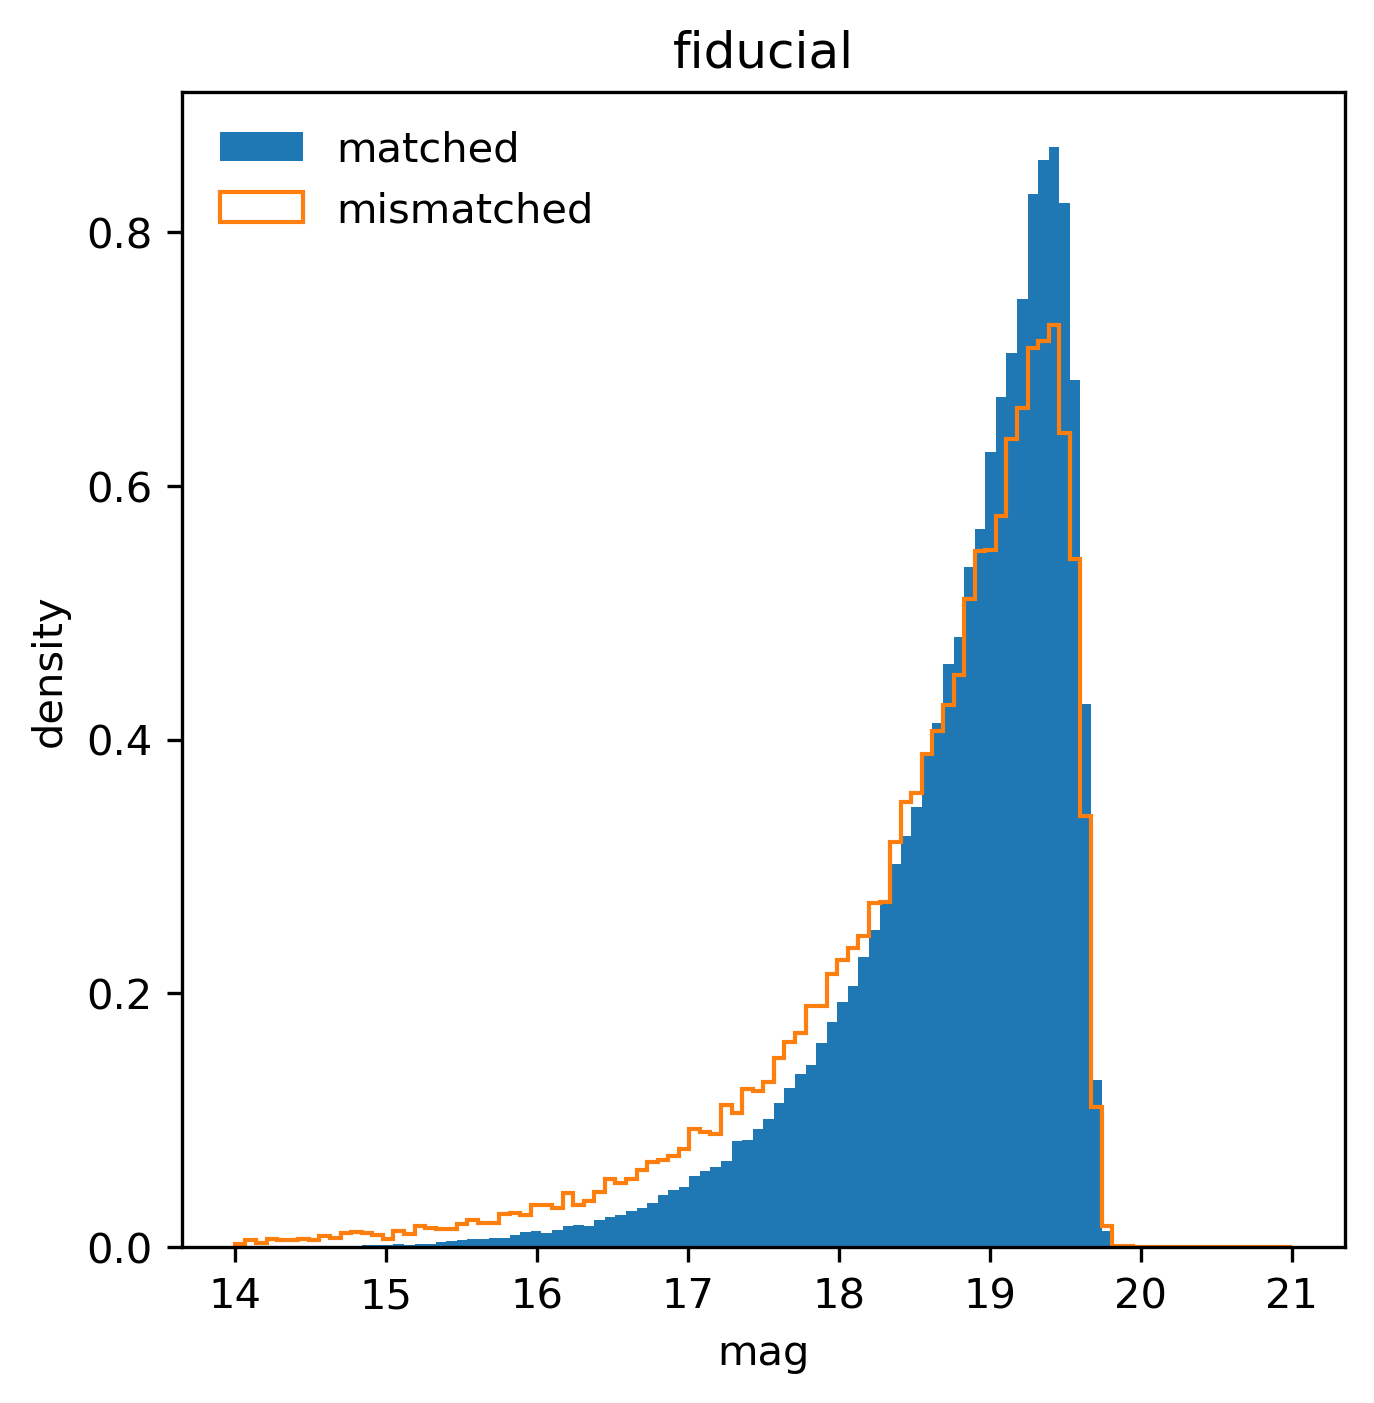
\includegraphics[width=0.45\linewidth]{figure/dr4_fiducial.png}
%         }
%     \subfigure[refined sample]{
%         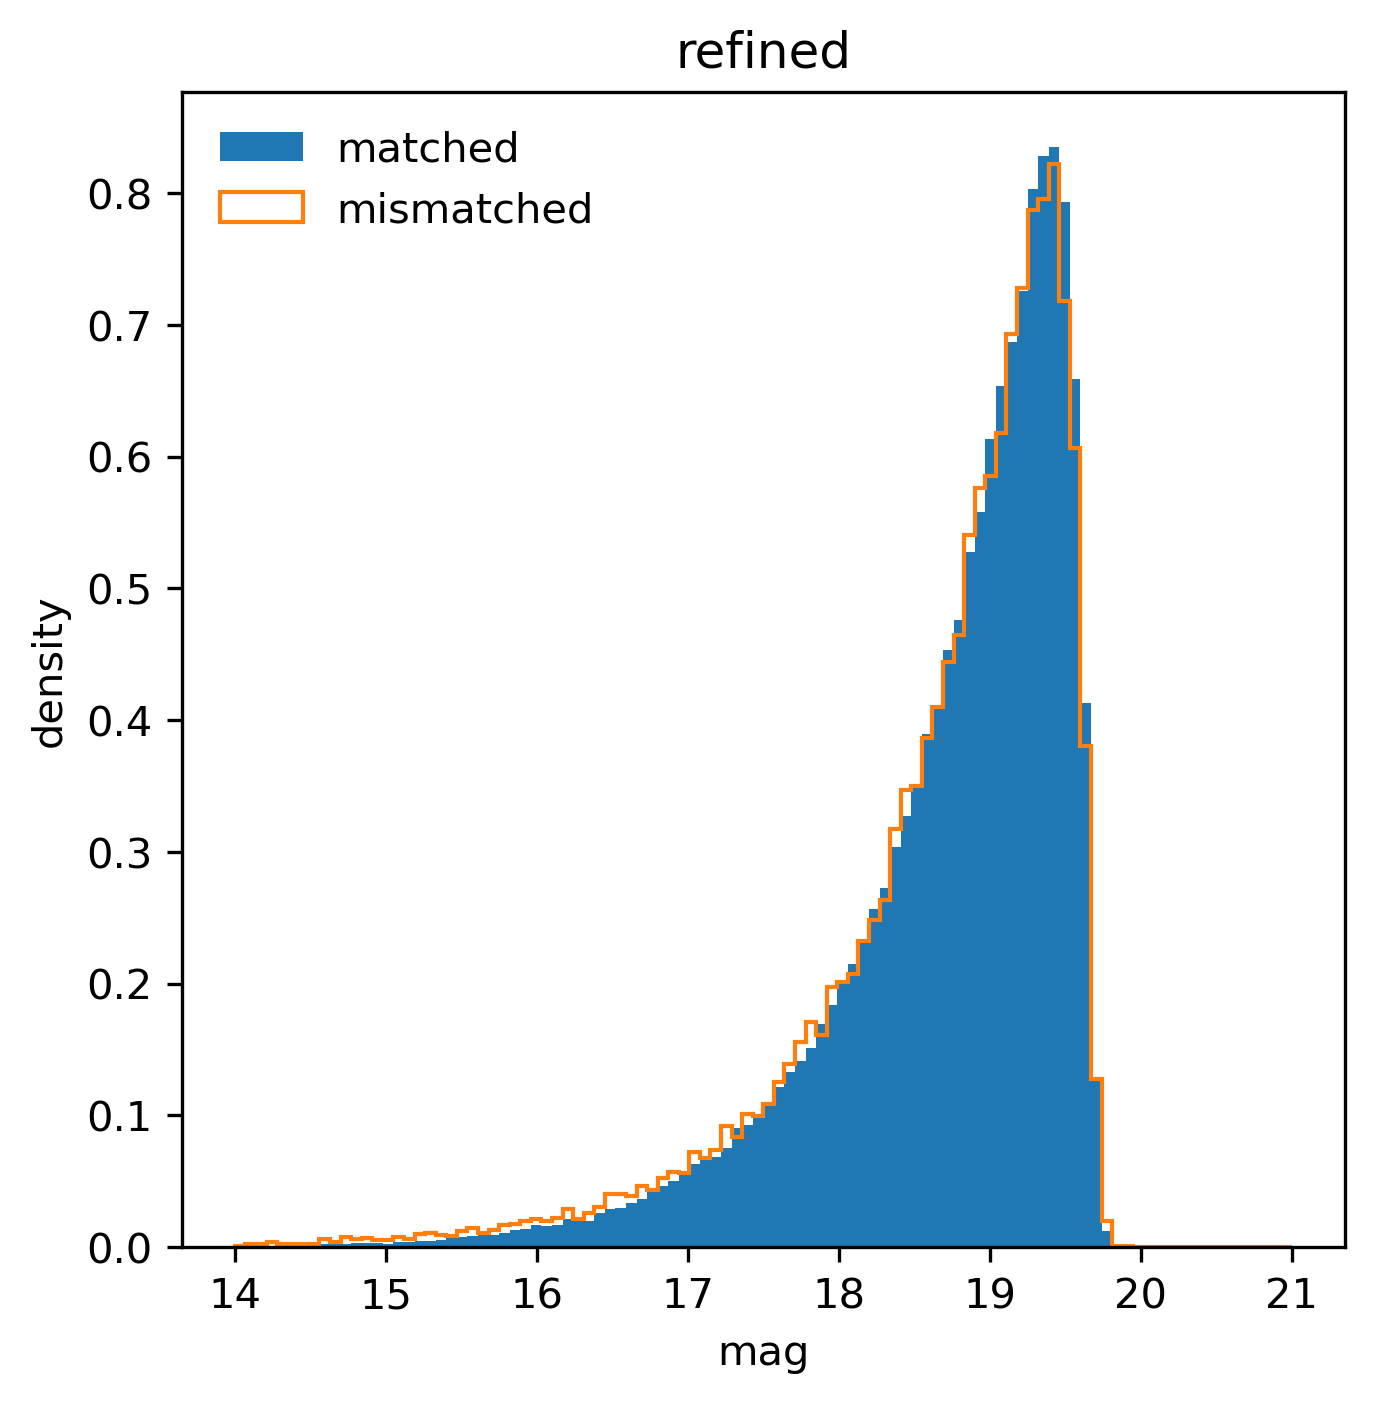
\includegraphics[width =0.45\linewidth]{figure/dr4_completed.png}
%     }
%     \caption{The distribution in magnitude of GAMA galaxies that are contained or missed in fiducial KiDs DR4 2DPHOT structural parameter catalogue or our refined catalogue.The yellow histogram shows the distribution in r-band magnitude of missed galaxies while the blue ones shows the galaxies that are contained.   }
%     \label{fig:example}
% \end{figure*}
% \par To complete the catalogue, we first find the galaxies that are excluded and add them to the KiDs structural catalogue, made our 'refined catalogue'. Although there're still some galaxies that can' t be found in KiDs catalogue, the distribution of those galaxies shows no feature of preference(Fig~\ref{fig:example} bottom). This mismatch could be the consequence of some artefact in original SDSS photometry and has already been observed by \cite{bellstedt_galaxy_2020}, which we don't necessary to worry about.
\begin{figure*}
    \centering
    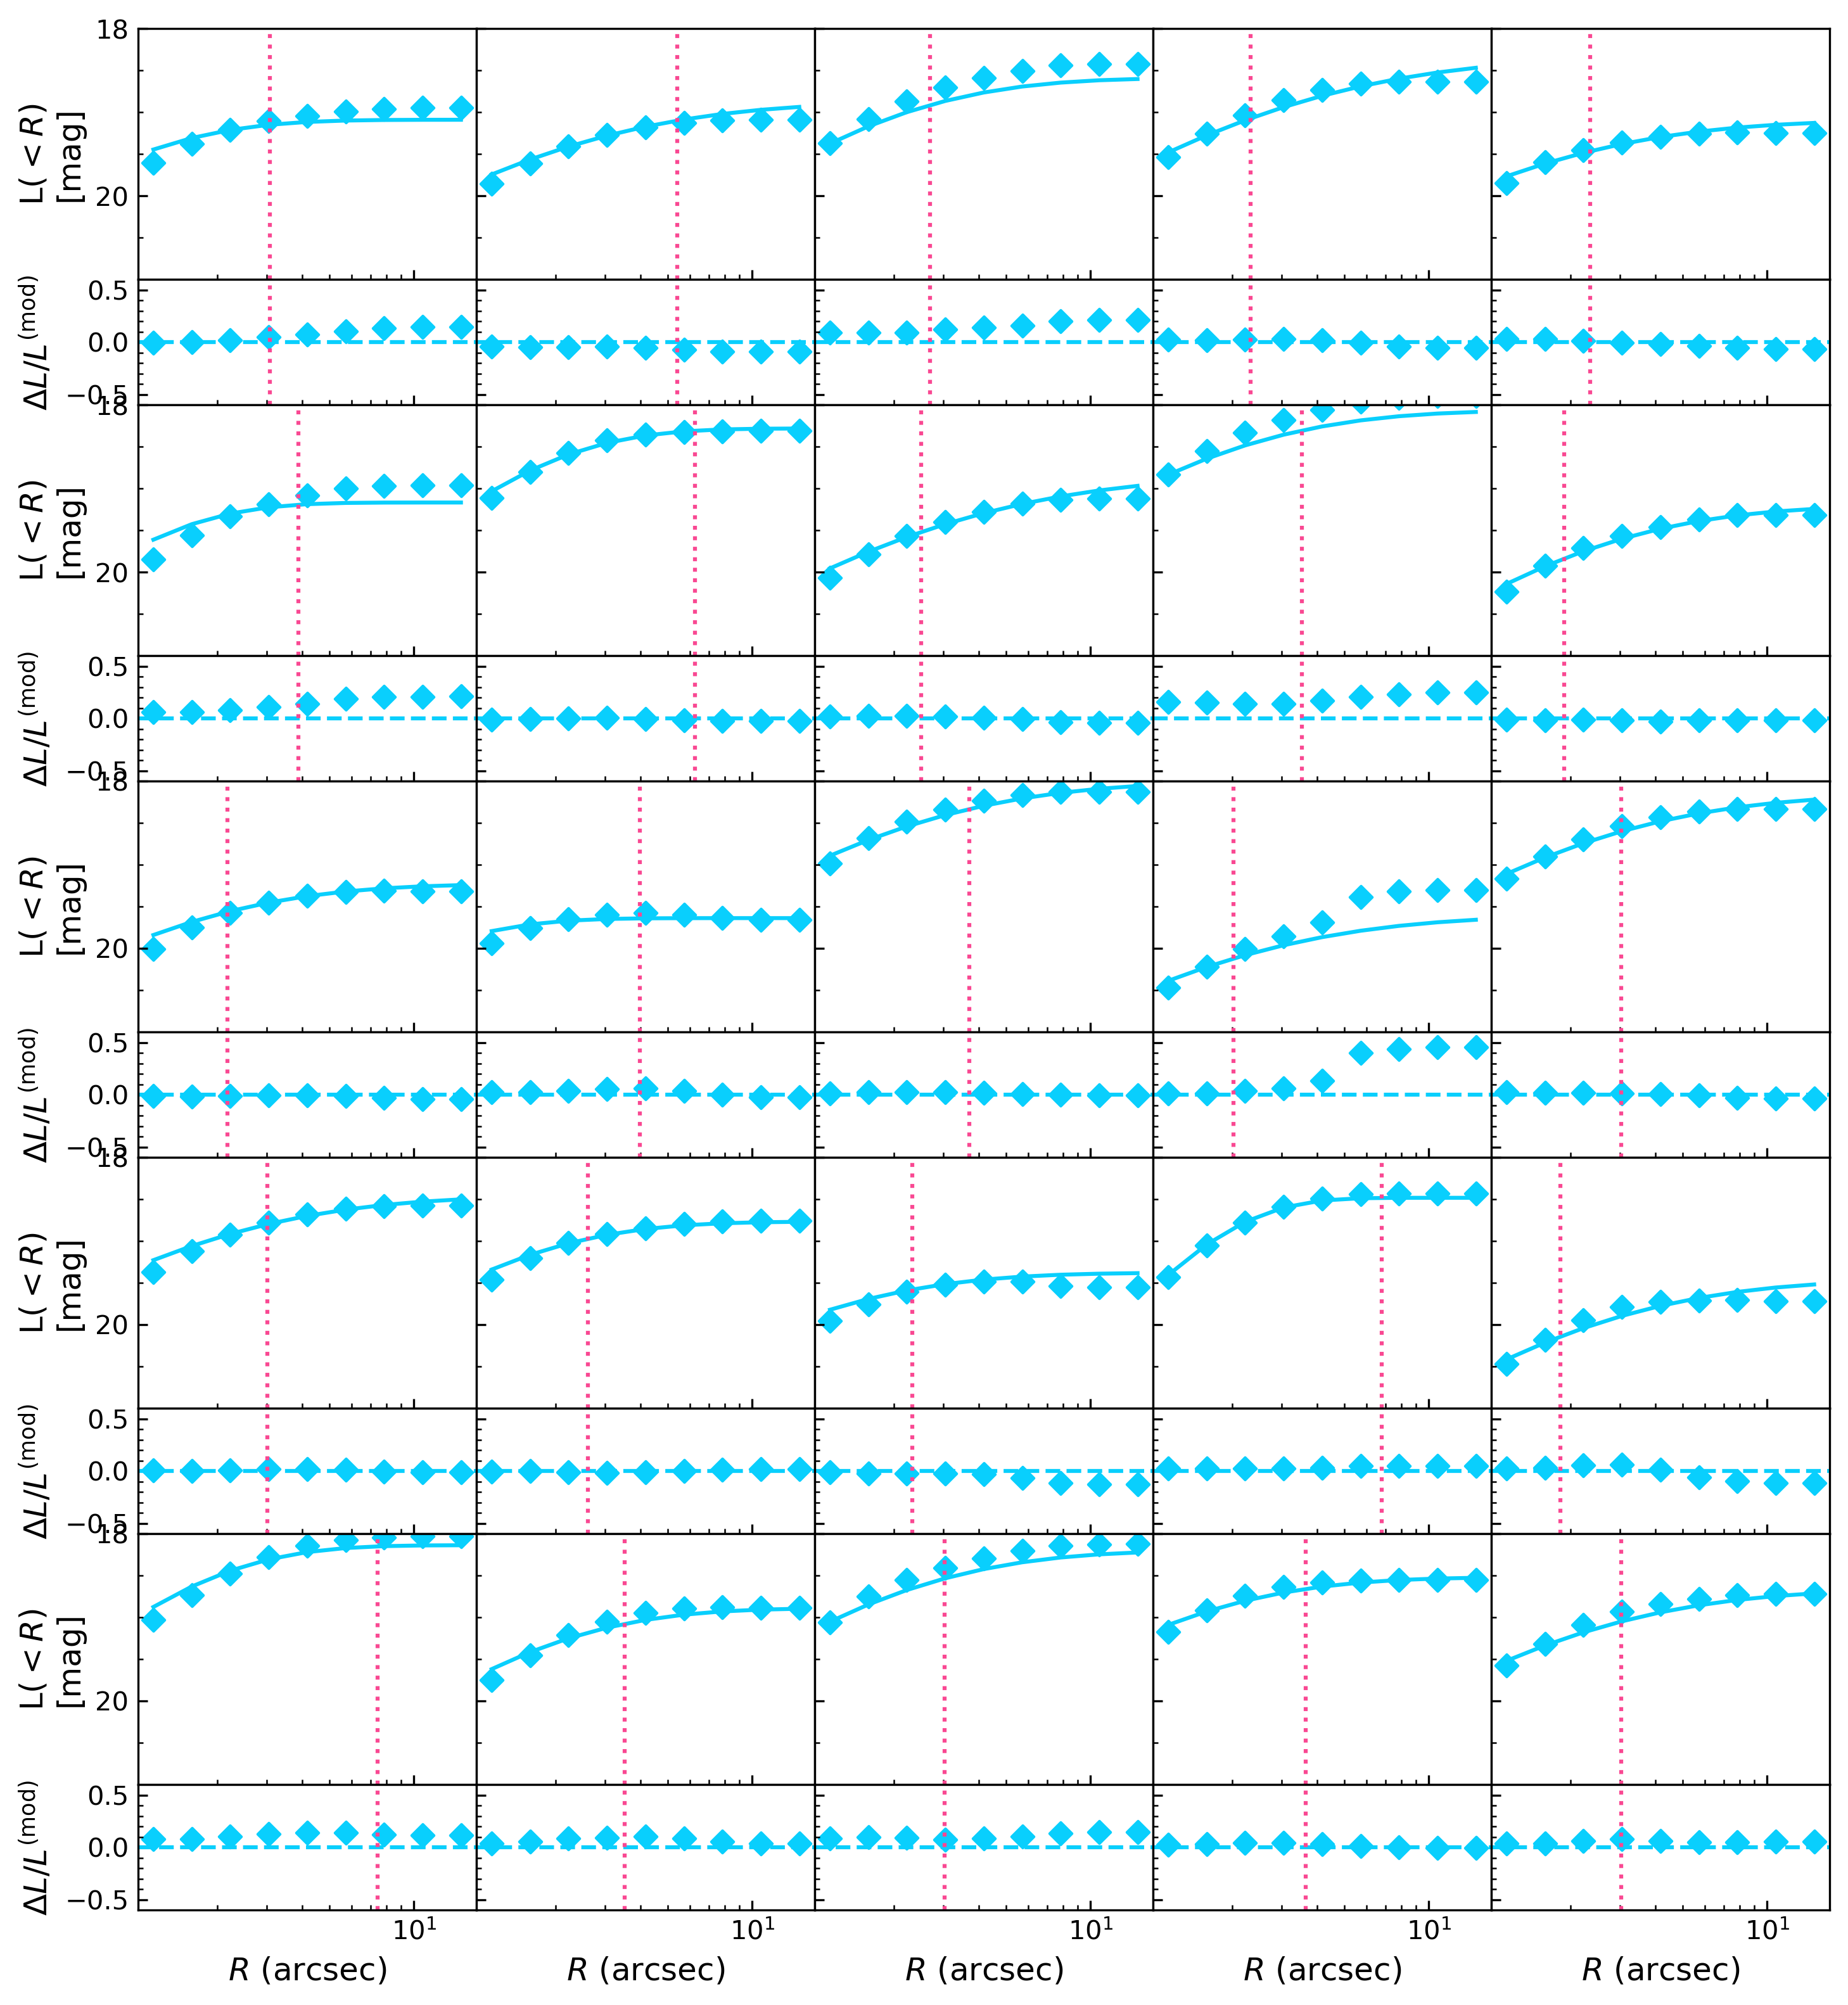
\includegraphics[width=0.8\linewidth]{figure/enclosed_mag.png}
    \caption{The upper panel shows the enclosed magnitude within 10kpc aperture of 25 galaxies that are random selected from our sample. The blue solid line shows the best-fitting S\'{e}rsic model calculated using GalNet structural parameters, while the blue diamonds are directly measured from KiDs r-band image. The lower panel shows the difference between the two measurements. The vertical dashed cyan line shows the corresponding angular size of 10kpc of each galaxy.} 
    \label{fig:enclosed_magnitude}
\end{figure*}
\subsubsection{Surface brightness model}
% \par Although we have complete the sample with those excluded galaxies, these galaxies are lack of accurate structural parameters. Therefore we need to fit the surface brightness ourselves for those missed galaxies. 
\par In our fitting, we use S\'{e}rsic profile to model the surface brightness of galaxies :
\begin{equation}
    I(R) = I_0 exp\left\{-b_n\left(\frac{R}{R_e}\right)^{1/n}\right\}
    \label{SB}
\end{equation}
Here, $q$ is the axis ratio, $n$ is the S\'{e}rsic index while $R$ is the circularised radius
\begin{equation}
    R^2 = qx^2 + \frac{y^2}{q}
\end{equation}
where $x,y$ are Cartesian coordinates, located at the center of galaxies. We use symbol $x$ to denote the axis that is aligned with the semi-major axis of the ellipse, while using $y$ to denote axis aligned with semi-minor axis. The effective radius $R_e$ is circularised as well.
\par Integrating Eq.\ref{SB}, we can obtain the light enclosed in a certain aperture $L(<R)$ (or the total light $L_{tot}$)
\begin{equation}
    L(<R) = 2\pi n\cdot I_0R_e^2 \cdot \frac{1}{\left(b_n\right)^{2n}}\cdot \gamma\left[2n,b_n \left(\frac{R}{R_e}\right)^{\frac{1}{n}}\right]
\end{equation}
\begin{equation}
    L_{tot} = 2\pi n\cdot I_0R_e^2 \cdot \frac{1}{\left(b_n\right)^{2n}}\cdot \Gamma\left(2n\right)
\end{equation}
Here $\Gamma$ is the gamma function, $\gamma$ is the lower incomplete gamma function and $b_n$ is a constant that ensure the light enclosed within the effective radius $R_e$ is a half of the total light.
\begin{equation}
    L_{tot} = 2 L(<R_e)
\end{equation}
Therefore, $b_n$ can be calculated by solving
\begin{equation}
    \Gamma(2n) = 2\gamma(2n, b_n)
\end{equation}

% \par The effective radius provided in fiducial catalogue has already been circularised, while GALFIT actually measured the effective radius $r_e$(use lowercase to denote the value measured by GALFIT) along semi-major axis, hence we need to convert it to circularised radius by 
% \begin{equation}
%     R_e = r_e \times \sqrt{q}
% \end{equation}
% \par We use the sky-subtracted and coadd science image in r-band (in consistent with fiducial sample) and using software SEXTRACTOR(\cite{Bertins_1996_Sextractor}) to mask the neighbouring objects with 1.5$\sigma$ detection threshold. The uncertainty of the sky is provided in the weight image, we then add the poisson noise calculated form the science image in quadruple and thus create the sigma image. We then ran GALFIT(\cite{Peng_galfit_2002}) and obtained S\'{e}rsic parameters for those missed galaxies.
% \par Combining with the S\'{e}rsic fitting result from KiDs DR4 structural catalogue, we obtained a sample within which all galaxies has reliable S\'{e}rsic parameters.We use 'refined sample' to represent this sample. 
\par In fact, galaxies may have various component, hence single S\'{e}rsic model might not be able to give a accurate description of the entire surface brightness profile. However, as we are focusing on the inner region of the galaxy, our only requirement is just the surface brightness in the inner region of galaxy can be accurately described by model.Therefore, we compared the profile of the enclosed light of galaxies with their best-fitting S\'{e}rsic model in Fig~\ref{fig:enclosed_magnitude} . We can easily observe that although some model do have discrepancy at some large radii, the enclosed light within $10kpc$ is still well constrained by model. 
\subsubsection{$M_{*,10}, \Gamma_{*,10}$ Calculation}
\label{sec:cal}
In our work, we assume that there is no mass-to-light ratio gradient inside one galaxy, hence the mass profile can be easily obtained via the light profile. We have obtained the stellar mass estimate for each galaxy from GAMA together with the light they use in the SPS model fitting process \citep{GAMAmain}, which enable us to calculate the mass-to-light ratio $\Upsilon$. The mass profile can be easily obtained by multiplying Eq3 and Eq4 with that $\Upsilon$.
\begin{gather}
    \Sigma_*(R) = \Upsilon I_0 exp\left\{-b_n\left(\frac{R}{R_e}\right)^{1/n}\right\} \\
    M_*(<R) = \Upsilon 2\pi n\cdot I_0R_e^2 \cdot \frac{1}{\left(b_n\right)^{2n}}\cdot \gamma\left[2n,b_n \left(\frac{R}{R_e}\right)^{\frac{1}{n}}\right]
\end{gather}
\par Simply substitute $R = 10kpc$ to Eq9, we obatined $M_{*,10}$, while $\Gamma_{*,10}$ is obatained by substituting Eq8 to Eq1. 
\subsection{Completeness}
To accurately measure the evolution of $M_{*,10}$ and $M_{*,10} - \Gamma_{*,10} $ relation, we do not expect any bias be introduced during the sample selection procedure. Therefore, we need our sample to be complete in $M_{*,10}$. Our fiducial sample is flux-limited, with its 95\% completeness limit down to r-band magnitude 19.65. To obtain a $M_{*,10}$ complete sample, we need to translate this completeness limit in magnitude to limit in $M_{*,10}$.
% \par GAMA provide the stellar mass estimation together with the r-band flux from SPS fit in its stellar mass DMU(\cite{GAMAmain}). We hence calculate the fraction of these two value and obtain the mass-to-flux ratio $\Upsilon$. Then we use the S\'{e}rsic parameters($R_e,n,b_n$) and the magnitude from surface brightness fitting in our refined sample  and calculated the flux that is enclosed in 10kpc $F_{10}$. It's straightforward that we can just multiply these two quantities and get $M_{*,10} = \Upsilon \times F_{10}$.
\par Then we need to translate the r-band critical magnitude $r_{crit} = 19.65$ to one critical $M_{*,10}$, namely $M_{*,10}^{crit}$. In fact, at arbitrary redshift, the ratio between $M_{*,10}$ and the total flux $F$ always spread a relatively wide range. Here we made an assumption that the ratio $M_{*,10} / F$ depend neither on $M_{*,10} $ nor on $F$, meaning that this quantity only describe one overall nature of quiescent galaxies at one given redshift. We then make narrow redshift bins, calculate the mean and standard deviation of the mass-to-flux ratio $M_{*,10} / F$ and use Gaussian distribution to estimate the critical value $M_{*,10} / F|_{crit}$ ,where the cumulative probability reach $95\%$ .Mutiplying $M_{*,10} / F|_{crit}$ by the corresponding flux of $r_{crit}$, we obtained the $M_{*,10}$ limit at that redshift bin. 
\begin{figure}
    \centering
    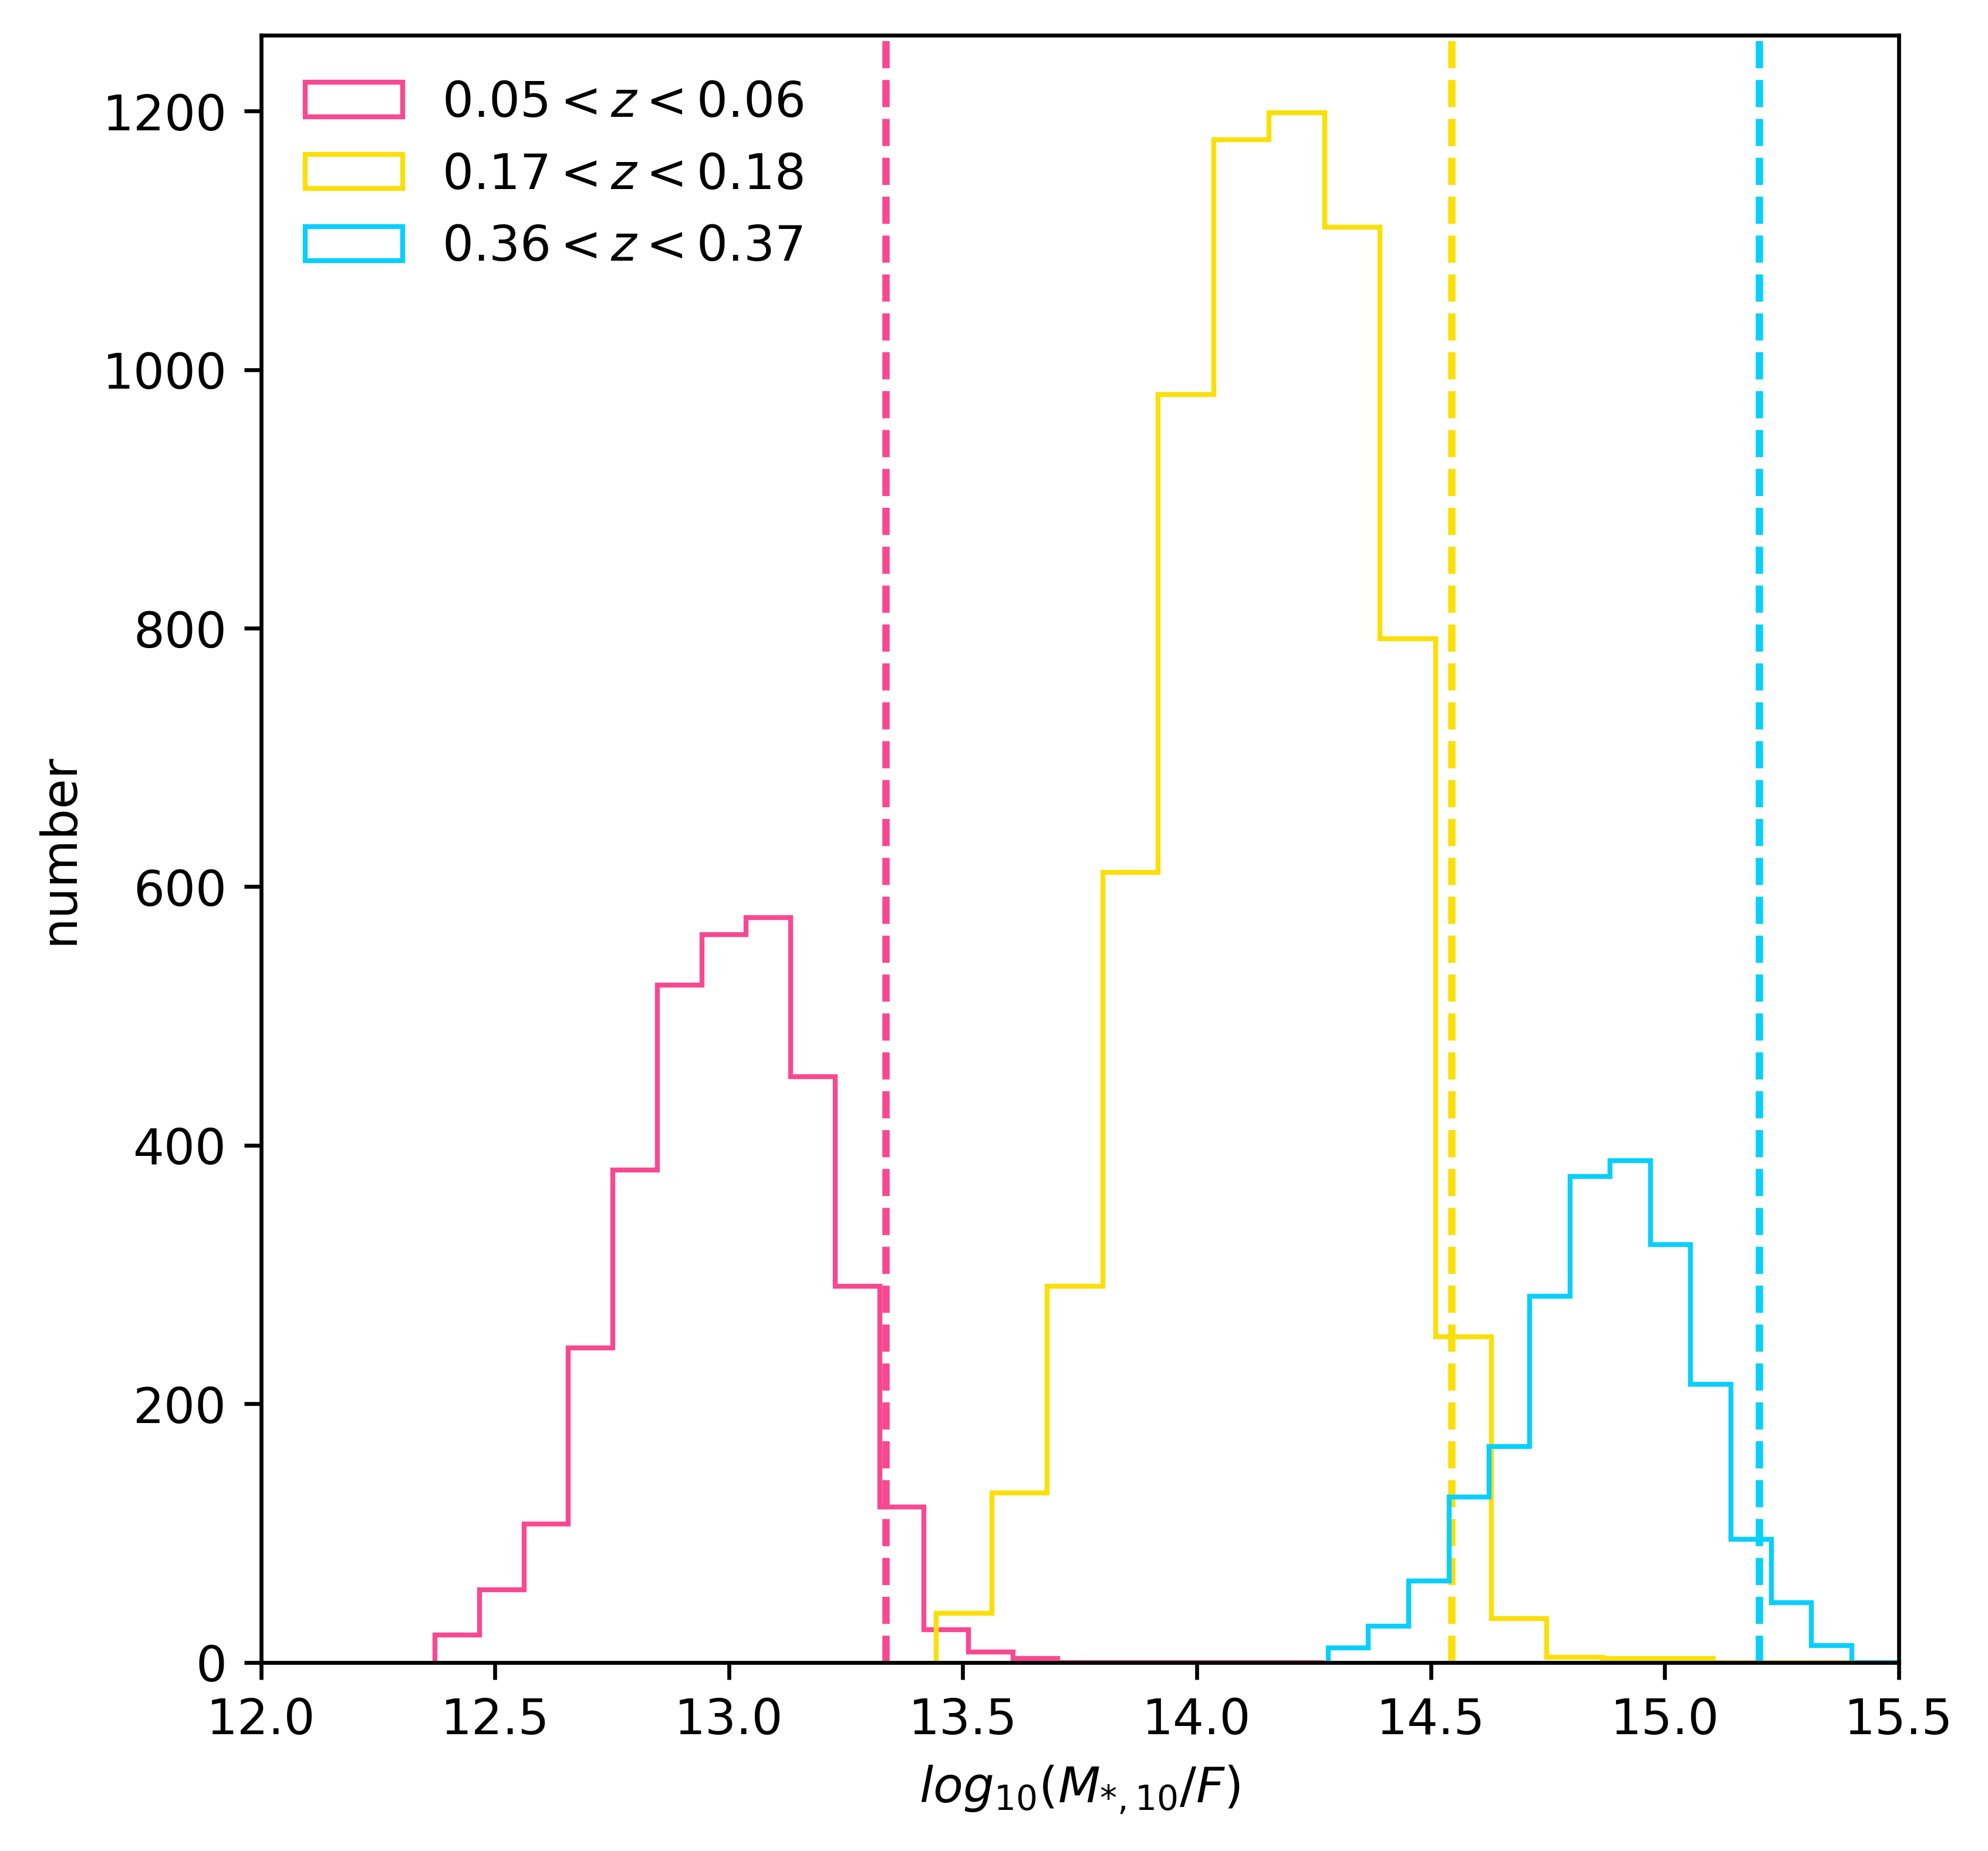
\includegraphics[width=\linewidth]{figure/m2f_ratio.png}
    \caption{The distribution of $M_{*,10} / F$ in three different narrow redshift bins. The vertical dashed line marks the $95\%$ percentile distribution in each bin.Mutiply this ratio by the flux corresponding to the r-band magnitude limit $r_{crit} = 19.65$, we then obtain the $M_{*,10}$ limit at that redshift bin.}
    \label{fig:m2f}
\end{figure}
\par Fig~\ref{fig:m2f} illustrate the procedure, it shows the dsitribution of $M_{*,10} / F$ in three different redshift bins, with dashed line shows the $95\%$ percentile of each bin. Operate this procedure iterative in each redshift bin and exclude galaxies whose $M_{*,10}$ is lower that the limit, we obtained a sample with $95\%$ completeness in $M_{*,10}$ and is shown in Fig~\ref{fig:completeness_cut}
\begin{figure}
    \centering
    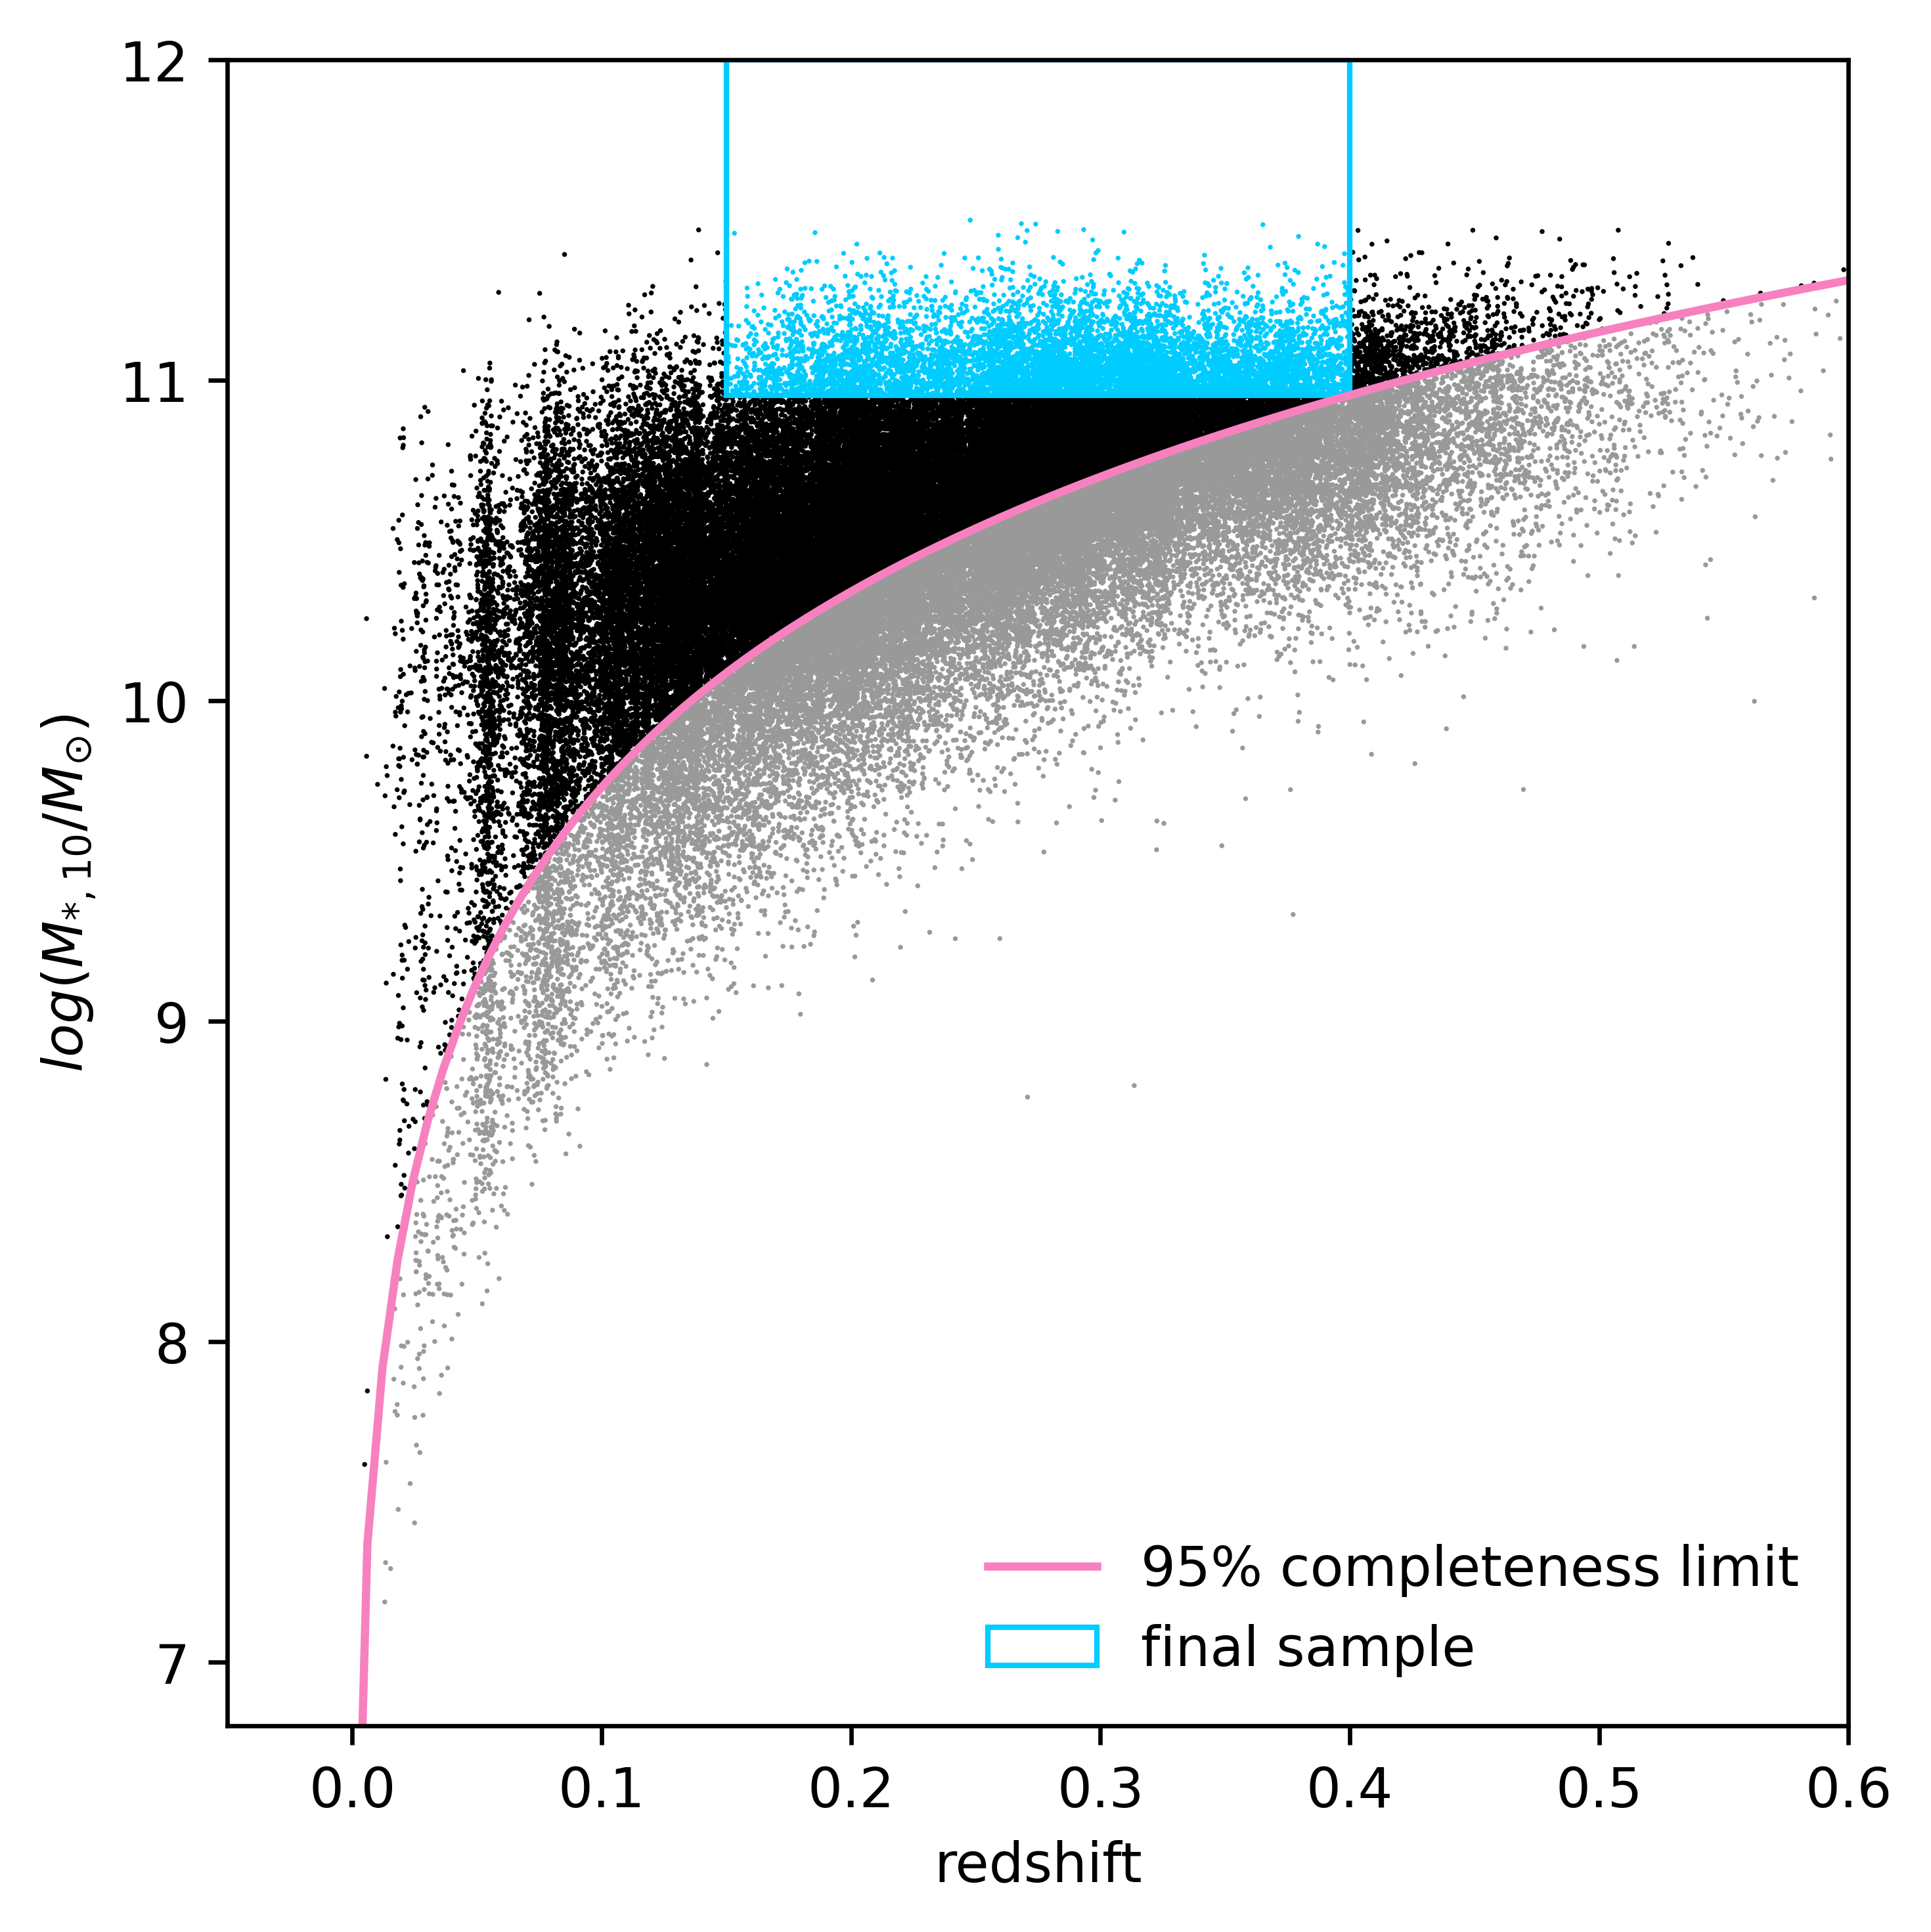
\includegraphics[width = \linewidth]{figure/completeness_cut.png}
    \caption{$95 \% $ completeness $M_{*,10} $ limit as a function of redshift of our ETG sample, shown in pink solid line.Galaxies above this pink line is adopted in our sample, shown in black dots, and the grey dots that lies below are those being excluded  }
    \label{fig:completeness_cut}
\end{figure}
% \par According to \cite{gallazzi_stellarmass_2009}, red galaxies has much narrower distribution of mass-to-light ratio than the blue one, hence the distribution of those red galaxies would be truncated at some stellar mass and the low mass end would be dominated by blue galaxies. This two population will mix with each other at higher stellar mass, exhibiting a nearly uniform color distribution. In Fig~\ref{fig:completeness_cut}, we can observe that our completeness has avoided those region that dominated by blue galaxies and selected the mixture of red and blue galaxies.
% In this paper, one basic assumption is the mass-to-light ratio is constant at arbitrary position of one galaxies.

% then used GALFIT(\cite{Peng_galfit_2002}) to fit a seeing convolved S\'{e}rsic model for those galaxies using r-band photometry. Neighbouring galaxies are masked using SEXTRACTOR (\cite{Bertins_1996_Sextractor})
% \subsection{GAMA Spectroscopy}
% In this work, we choose galaxies from GAMA DR4\citep{GAMAmain} with $Dn4000 > 1.5$, in order to choose ETGs, and then we've done a crossmatch with kiDs data. Given that the stellar-mass measurement of KiDs uses photometric redshift, we make use of the stellar mass catalogue provided by GAMA. We calculate the ratio between stellar mass and the derived r-band flux from the SPS fitting. We further assumed the "mass-to-flux" ratio is constant in a single galaxy, then we can use this value to calculate the stellar mass using the photometric data, specifically the r band magnitude, of KiDs'. 
% \par According to GAMA DR4\citep{GAMAmain}, the completeness of galaxies is less than $95\%$ for galaxies with r-band magnitude greater than $19.8$. We desire a complete sample in stellar mass, so we investigate the distribution of stellar mass in each redshift range with r-band magnitude equals to 19.8, in order to convert the completeness in magnitude to the completeness in stellar mass. The distribution is shown in figure 1. In various redshift, we find the stellar mass corresponding to the 95 percentile of the distribution and exclude the galaxies with lower stellar mass value.  

% \subsection{KiDs}
% In this work, we use the “2DPHOT structure parameter catalogue" in DR4-KiDs-1000(I'm not sure which paper to cite). After cross-matched with GAMA data, we first convert the r-band magnitude provided by this catalogue to the flux data. Then we use the "mass-to-flux" ratio calculated using GAMA data and obtain the self-consistent stellar mass for KiDs photometric data. 
% \par In addition to the photometric data, the catalogue also provided the Serisic parameters of each galaxy. Using these parameters, we are able to construct the surface brightness profile by
% \begin{equation}
%     I(R) = I_0exp\left \{-b(n\left(\frac{R}{R_e}\right)^{1/n}\right\}
% \end{equation}
% \par Here $R$ is the circulised radius $R^2 \equiv qx^2+ \frac{y^2}{q}$, where $q$ is the axis ratio. The "structure catalogue provided us the half-light radius $R_e$ and the S\'{e}rsic index $n$.$I_0$ is the surface brightness in the center of one galaxy and $b(n)$ can be calculated by constraining the region enclosed in the hald-light radius $R_e$ contains half of the total light.Hence, we can calculate the mass enclosed in $10kpc$($M_{*,10}$) and the mass-weighted projected surface brightness slope ($\Gamma_{*,10}$)
% \subsection{Completeness}
\subsection{Simulation}
In order to build a intuitive understanding of the growth in $M_{*,10}$ and $\Gamma_{*,10}$ due to mergers, we utilize a collection of 8 sets dissipationless binary-merger simulations which has been used in \cite{sonnenfeld2014} to construct a dry-merger model. These 8 sets of simulations has five different parameter settings and is reported in Table~\ref{tab:simulation}. 
Each set contains two simulations with nearly identical parameter settings except for their different orbital angular momentum in order to take both 'head-on' and 'off-axis' encounter into consideration. All orbits are parabolic.   
\begin{table}
    \centering
    \caption{Simulation parameters for different sets of simulation. }
    \label{tab:simulation}
    \resizebox{\columnwidth}{!}{
    \begin{tabular}{cccccccc}
        
        \hline
        % \hline
        Set & $\xi$ & $(M_h/M_*)_{\text{main}}$ & $C_{\text{main}}$ & $(r_s/R_{\text{eff}})_{\text{main}}$ & $(M_h/M_*)_{\text{sat}}$ & $C_{\text{sat}}$ & $(r_s/R_{\text{eff}})$ \\
        \hline
        D & 1.0,0.5,0.2 & 49 & 8.0 & 11.6 & 49 & 8.0 & 11.6 \\
        D1 & 0.5 & 49 & 5.0 & 11.6 & 49 & 5.0 & 11.6 \\
        D2 & 0.5 & 49 & 8.0 & 6.0 & 49 & 8.0 & 6.0 \\
        D3 & 0.2 & 49 & 8.0 & 11.6 & 35 & 8.5 & 8.8 \\
        D4 & 0.2 & 49 & 8.0 & 11.6 & 75 & 8.0 & 15.0 \\
        \hline
    \end{tabular}}
\end{table}
\par The two progenitors, i.e. main galaxy and satllite galaxy , in each set of simulation are spherical symmetric and are composed of dark matter halo and stellar component. The stellar profile can be decribed by $\gamma$ model (\cite{Dehnen93}; \cite{Tremaine94})
\begin{equation}
    \label{eq:profile_stellar}
    \rho_*(r) = \frac{3-\gamma}{4\pi}\frac{M_*r_*}{r^\gamma (r+r_*)^{4-\gamma}}
\end{equation}  
where $M_*$ is the total stellar mass. The simulation adopt $\gamma = 1.5$ . 
\par The dark matter halo is described by NFW profile (\cite{NFW})
\begin{equation}
    \label{eq:profile_halo}
    \rho_{DM}(r) = \frac{M_{DM,0}}{r(r+r_s)^2} exp\left[-\left(\frac{r}{r_{vir}}\right)^2\right]
\end{equation}
According to \cite{nipoti2009}, $r_s$ is the scale radius, while $M_{DM,0}$ is a reference mass. A exponential cut-off is adopted as a truncation of the halo, hence the total dark mass would not extend to infinity. As the summation of the two components, the total mass profile $\rho(r) = \rho_*(r) + \rho_{DM}(r)$ is nearly isothermal: the slope $\gamma'$ of the toal mass profile in 8 sets of simulation lies in the range of $1.97 \sim 2.03$.

\par The simulation is run with FVFPS code (Fortran Version of Fast Poisson Solver, \cite{londrillo03,nipoti03}) The following code parameter values are adopted: minimum value of the opening parameter $\theta_{min} = 0.5$ while the softening parameter $\epsilon = 0.04 R_\text{eff}$, here $R_\text{eff}$ represent the effective radius of the main galaxy. The timestep $\Delta t$ is the same for all particles, while is allowed to vary depending on the maximum particle density $\rho_{max}$ at that epoch.In particular, the timestep can be adapted by $\Delta t = 0.3/(4\pi G \rho_{max})^{1/2}$.The realisation of the initial condition is identical to that in \cite{nipoti2009}, with the mass of dark matter parts twice as heavy as stellar particles.
% \par As the origin simulation data didn't give a physical unit of both mass and radius, we now have the freedom to 'rescale' the simulation data to generate galaxies with different size and mass. In practise, we modify the remnant galaxy with three different length unit so that the effective radius $R_e$ of the remnant galaxy equals to $1.22,5,10 kpc$.  
% \section{Method}
% \subsection{Random catalogue}
% Obtaining the $M*_{,10}$ and $\Gamma_{*,10}$ data, we want to plot the $M_{*,10}$ function and investigate its redshift-dependent evolution ,which require us to know the effective volume of our sample. Here we apply the random catalogue method to investigate such issue........
% \subsection{Beyesian hierarchical method?}

\section{Result}
\subsection{The growth of $M_{*,10}$ and $\Gamma_{*,10}$ in simulation}
In order to investigate the growth of these two parameters, we only need to focus on two snapshots of the simulation. The first snapshot is the initial state which contains the initial main galaxy and satellite galaxy, in fact, we only care about the main galaxy. The second snapshot is the final state when the merging process is finished leaving a remnant galaxy. The word 'finish' means that the remnant stellar system is relaxed and virialised, while the remnant galaxy is the collection of dark matter particles and stellar particles that are bounded. We project the initial and remnant galaxies onto x-y plane so as to generate a mock observational image of these two, the mock image is shown in Fig.\ref{fig:mock_image}.The initial main galaxy is spherical, thus its image is a circle. In contrast, the remnant galaxy does not have this symmetry, hence we can observe that its image is a ellipse. In order to make a fair comparison, we then circularised the remnant ellipse. In particular, we measured the quadruple moment of the remnant galaxy image, and then stretch and rotate the image according to this quadruple moment until the image become a circle.
\begin{figure}
    
    \centering
    \includegraphics[width=\linewidth]{figure/circularised.png}
    \caption{\label{fig:mock_image}In this plot I choose the simulation set D3 to illustrate the mock images of main and remnant galaxies. The left panel shows the  initial main galaxy, while the middle and right panels are  the uncircularised and circularised remnant galaxy respectively. The unit is in code unit, instead of physical unit}
\end{figure}
Having done this circulrisation, we are enabled to measure the $M_{*,10}$ and $\Gamma_{*,10}$ of both circularised initial main galaxy and circularised remnant galaxy, and make direct comparison to see how these two quantities grow during the merging process.
\par Actually, the mass,length, time and velocity are not in physical unit, but in code unit. That means we have the freedom to 'rescale' the simulation data, i.e. specify a physical value for these 'code unit', to generate galaxies with different size and mass. Traditionally, changing the mass and length unit may affect the timestep used in the simulation, but as we only focus on two snapshots and ignoring the time that one merger event take, we believe this 'rescale' operation would not severely affect our result. The default scale of the simulation set the length unit to $1 kpc$ and the total stellar mass of the main galaxy is $log_{10}(M_*) = 10.5$ so that the effective radius of which is $R_e = 1.22 kpc$. We then make two other modification to make the initial main galaxy has $R_e = 5,10 kpc$, meaning that the physical value of one code length unit is $4.1, 8.2 kpc$ respectively in each modification.Therefore, for each set of simulations, we have three pairs of main and remnant galaxies. We then measured the $M_{*,10}$ and $\Gamma_{*,10}$ of all six galaxies in one set for all sets of simulations. The result is shown in Fig.\ref{fig:sim_result}. 
\begin{figure}
    \centering
    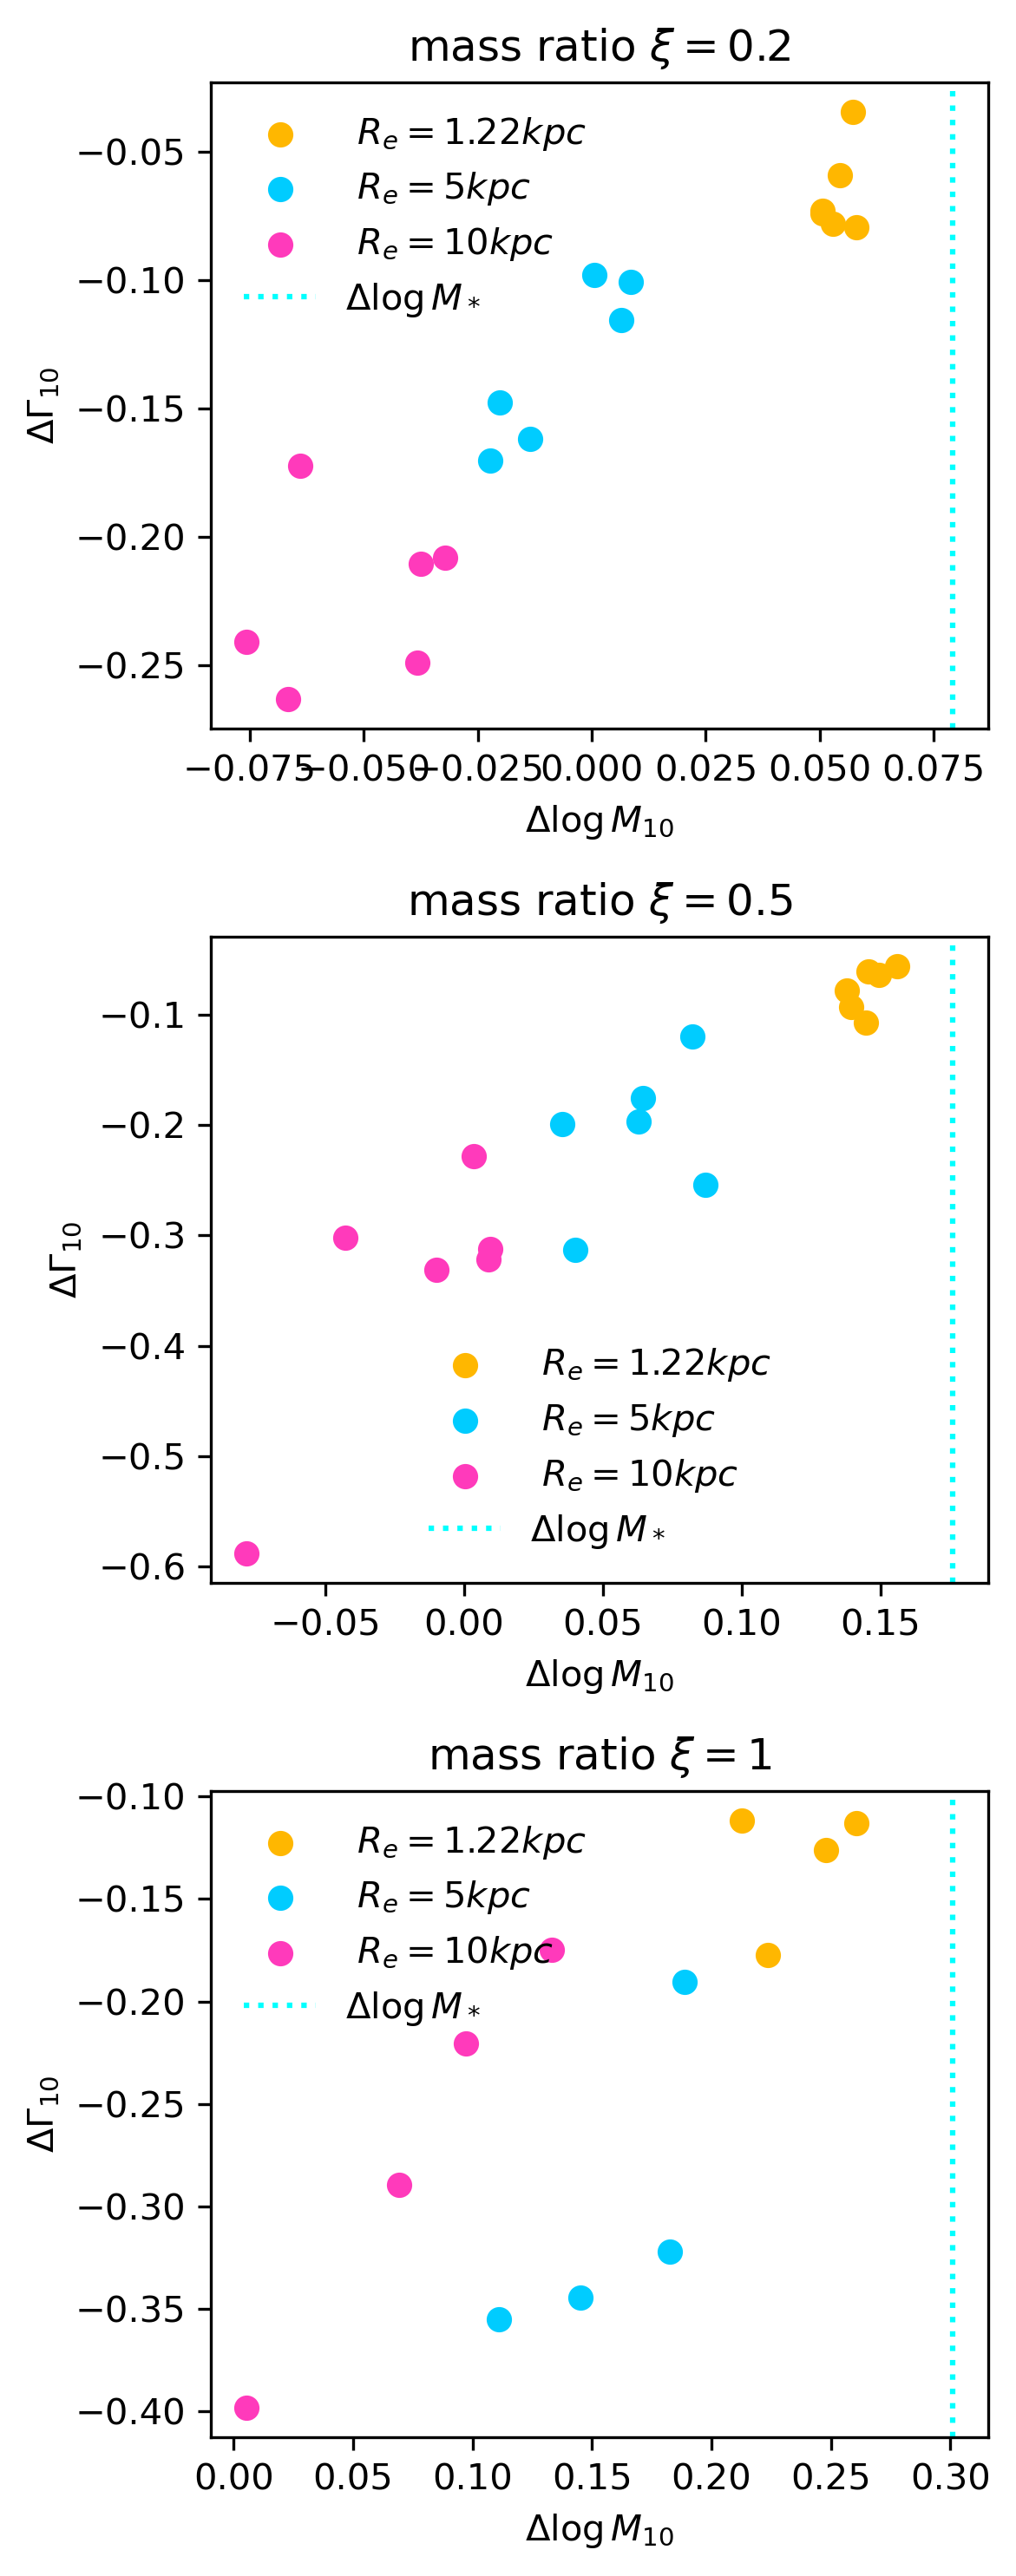
\includegraphics[width=0.75\linewidth]{figure/sim_result.png}
    \caption{ Three panels show the change in $logM_{*,10}$ and $\Gamma_{*,10}$ due to mergers with three different merger ratio $\xi$, while the three colors represent different initial effective radius $R_e$ of the main galaxy.The vertical dotted cyan line shows the logarithmetic change in the total stellar mass for each merger ratio. }
    \label{fig:sim_result}
\end{figure}
\par We can easily observe that for all three merger ratios, the parameter $\Gamma_{*,10}$ always shows a decreasing trend, while for larger, more massive galaxies, the decrease in $\Gamma_{*,10}$ tends to be more significant. On the other hand, the growth of parameter $log M_{*,10}$ is a bit more complicated. In general, the growth in $log M_{*,10}$ is always less than the growth in the total stellar mass $\log M_*$, which may indicating that larger fraction of accreted mass are sunk in the outer region of the galaxy. In contrast with the $\Gamma_{*,10}$, smaller galaxies show a larger increase in $log M_{*,10}$. Interestingly, if one pay more attention to the first two panels (top and middle panel), one can find that in some cases, the growth in $log M_{*,10}$ could be even negative after the merger. While for the largest merger ratio $\xi = 1.0$ (bottom panel), the growth in $log M_{*,10}$ is always positive. The negative value informs us that the merger do varies the entire density profile of the galaxy, and the inner region of galaxies may experienced the most significant change comparing with the outer region.The impact on the inner region of galaxies tends to be stronger for mergers with smaller mass ratio.Small mass ratio minor-mergers may flatten the density profile, puffing-up the galaxies hence make $log M_{*,10}$ decrease and $\log M_*$ increase simultaneously.
\subsection{Observation result}
\par Having investigate the result in simulations, we then operate the measurement to our observation sample. In fact, we have done a small modification on the total stellar mass. In case that we use the stellar mass measured by GAMA survey and use S\'{e}rsic parameter measured by KiDs survey, the flux of one single galaxy that has been used in the measurement of these two surveys may not be consistent. Here we made the assumption that the mass-to-flux ratio is a constant value in one single galaxy and calculated this ratio $\Upsilon$ for each galaxy, using the data of total flux (converted from apparent magnitude) and stellar mass in GAMA survey. We then multiplied this ratio by the total flux measured by KiDs survey and obtained the stellar mass that is in consistent with the KiDs S\'{e}rsic parameter.  
\par As a consequence of the completeness cut, galaxies with lower $M_{*,10}$ value at higher redshift would be absent in our sample. To investigate the evolution trend in $M_{*,10 } - \Gamma_{*,10}$ relation, we have to either narrow the redshift range to include more low-$M_{*,10}$ galaxies or narrow the $M_{*,10}$ range to include more high-redshift galaxies. In this work, we choose the latter one, meaning that we only focus on massive quiescent galaxies whose $M_{*,10} \geq 10^{10.9} M_{\odot}$. In addition, we set a lower limit on the redshift range $ z \geq 0.15$. It's easy to observe some vertical stripe-like feature in Fig.\ref{fig:completeness_cut} at low redshift end, and is thought to be the effect of large scale structure by \cite{GAMAmain}. It is reasonable as the comoving volume at low redshift is relatively smaller, so it is more likely to suffer from cosmic variance. We thus determined this low-redshift cut in order to avoid such cosmic variance. The final sample we used to investigate the evolution is show by cyan dots in Fig.\ref{fig:completeness_cut}. We binned the sample in redshift and $M_{*,10}$, then calculated the median value of $\Gamma_{*,10}$ in each bin. The $\Gamma_{*,10}$ result is shown as a function of $M_{*,10}$ in Fig.\ref{fig:mg_relation} and as a function of redshift in Fig.\ref{fig:gamma}.
\begin{figure}
    \centering
    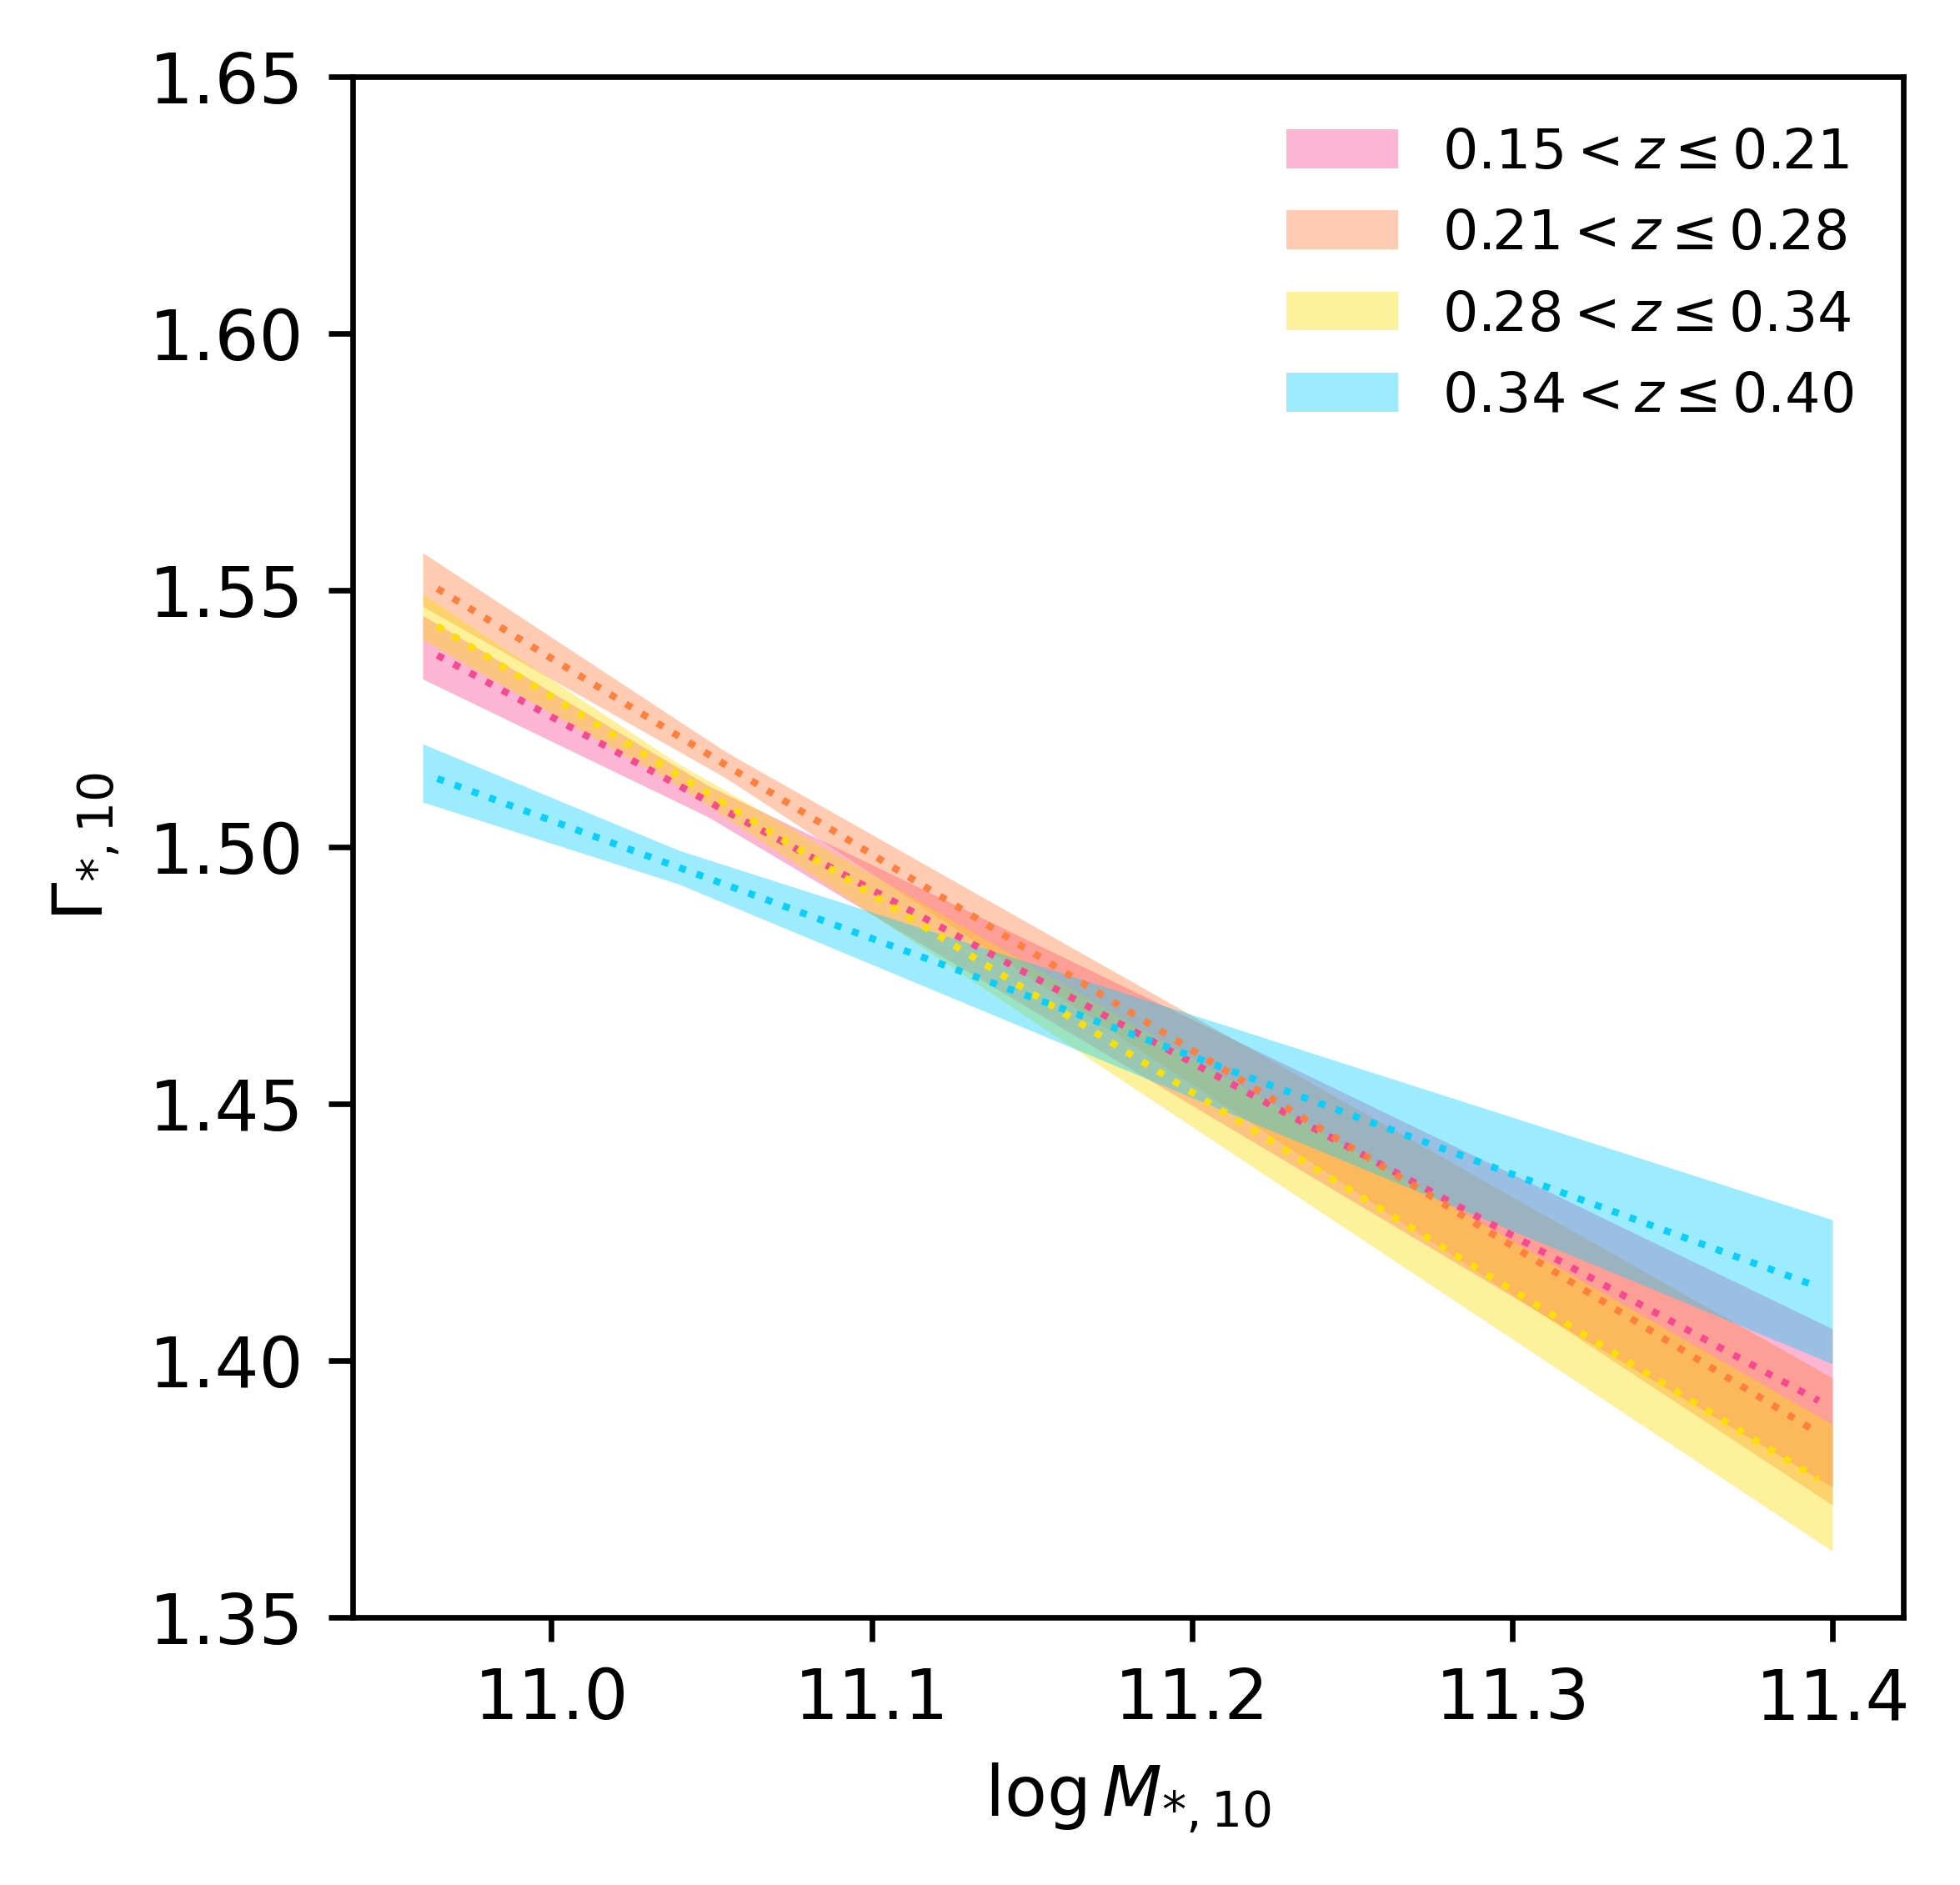
\includegraphics[width=\linewidth]{figure/mg_relation.png}
    \caption{The $M_{*,10} - \Gamma_{*,10}$ relation of our observation sample. The sample are divided into four redshift bins, and are shown in different colors. The error bar represents the standard error in each bins.}
    \label{fig:mg_relation}
\end{figure}
\begin{figure}
    \centering
    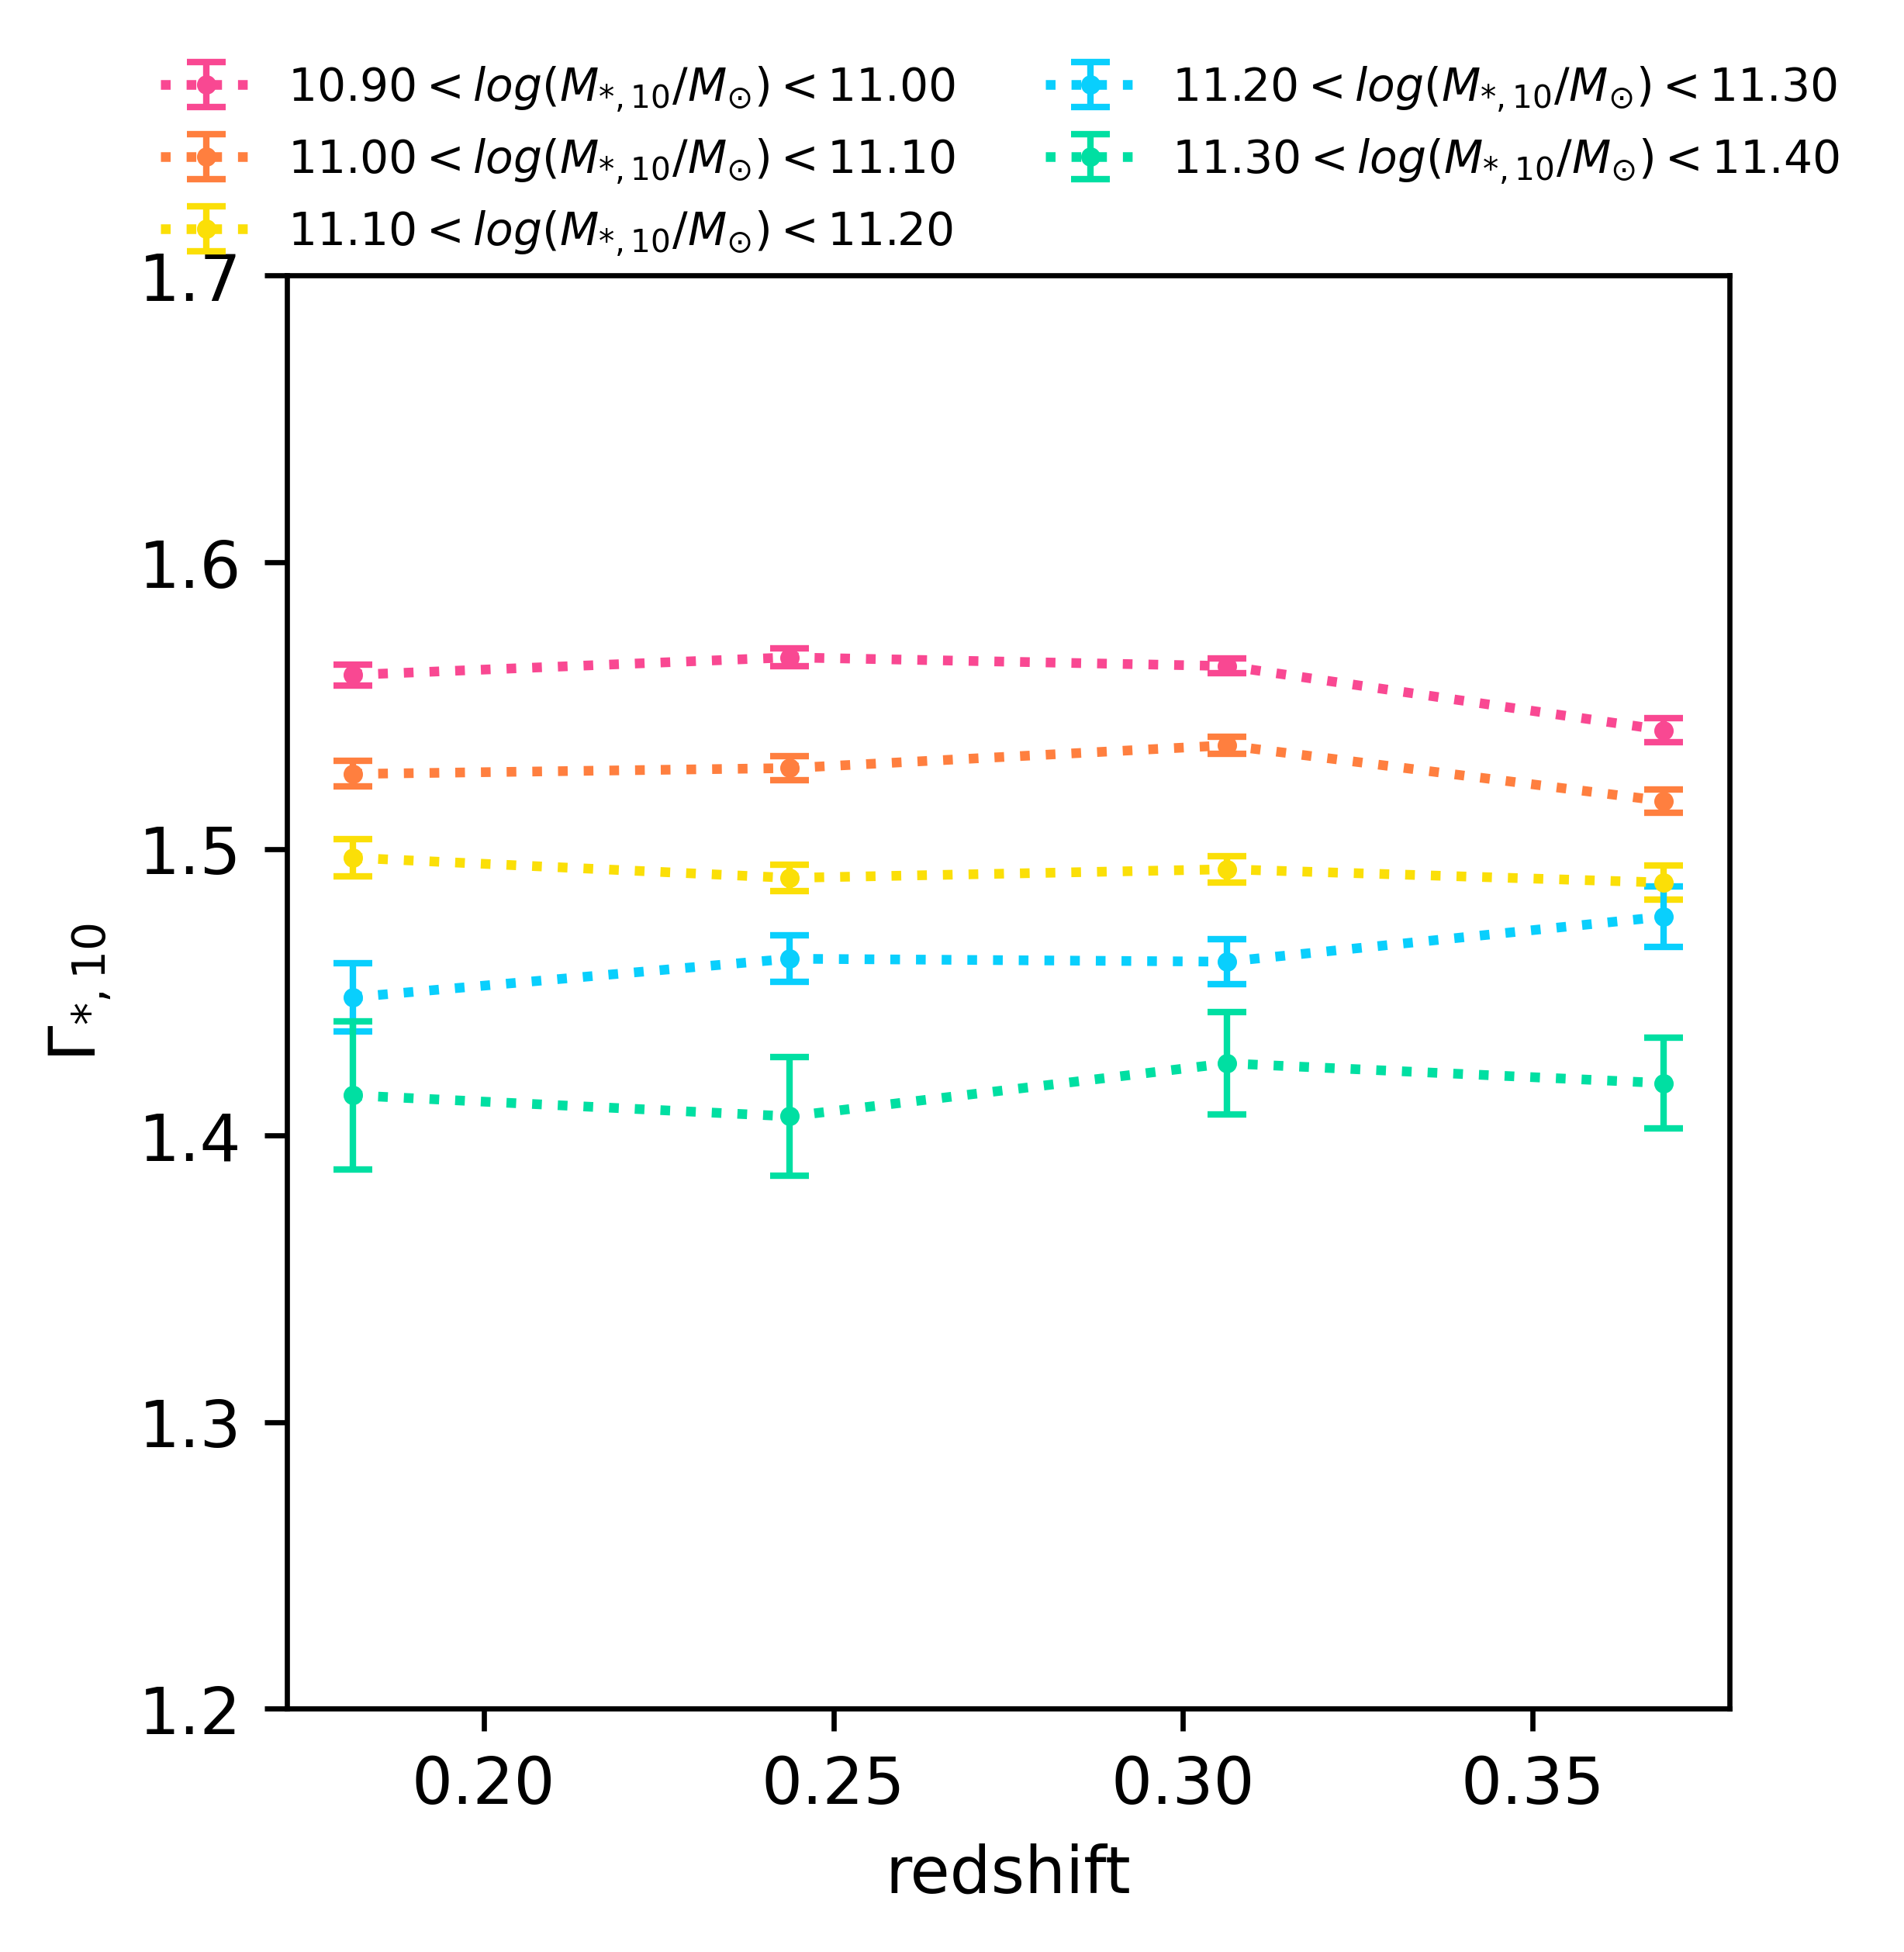
\includegraphics[width=\linewidth]{figure/gamma.png}
    \caption{$\Gamma_{*,10}$ as a function of redshift in each $M_{*,10} $ bin. The sample are divided into five different $M_{*,10}$ bins.The error bar represents the standard error in each bins.}
    \label{fig:gamma}
\end{figure}
\par In Fig.\ref{fig:mg_relation}, we could observe a anti-correlation between $M_{*,10}$ and $\Gamma_{*,10}$. Comparing the data in four redshift bins simultaneously, we can hardly see the evolution trend in this relation. In addition, if we focus on $\Gamma_{*,10}$ only, as shown in Fig.\ref{fig:gamma}, we could reach a similar conclusion that there is no significant evolution in $\Gamma_{*,10}$.The $\Gamma_{*,10}$ value in five different $M_{*,10}$ are all almost constant as the redshift grows. The error bars in these two plots are standard error in each bin, i.e the standard deviation divided by the square root of the number of galaxies in each bins. The error bar is relatively larger at higher $M_{*,10}$ end, but it does not affect our conclusion as in Fig \ref{fig:mg_relation}, the data points are still overlapping with each other in the same $M_{*,10}$ bin and the $\Gamma_{*,10} - z$ relation can still be reckoned as a horizontal line. 
% a: 
% Figures and tables should be placed at logical positions in the text. Don't
% worry about the exact layout, which will be handled by the publishers.

% Figures are referred to as e.g. Fig.~\ref{fig:example_figure}, and tables as
% e.g. Table~\ref{tab:example_table}.

% % Example figure
% \begin{figure}
% 	% To include a figure from a file named example.*
% 	% Allowable file formats are eps or ps if compiling using latex
% 	% or pdf, png, jpg if compiling using pdflatex
% 	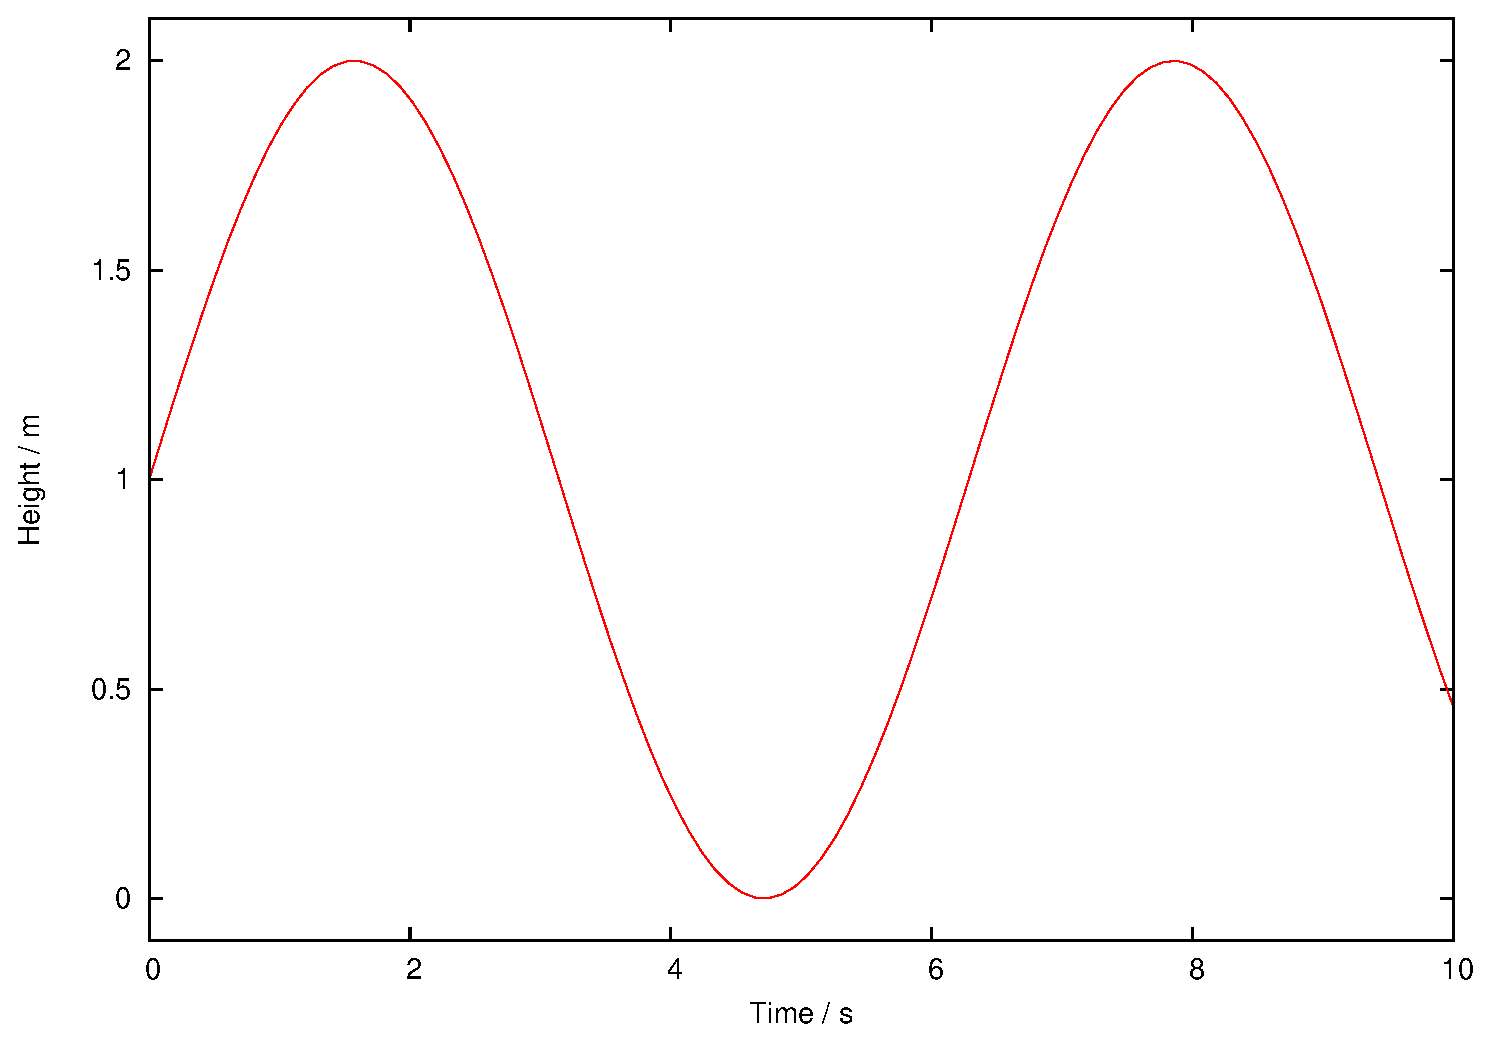
\includegraphics[width=\columnwidth]{example}
%     \caption{This is an example figure. Captions appear below each figure.
% 	Give enough detail for the reader to understand what they're looking at,
% 	but leave detailed discussion to the main body of the text.}
%     \label{fig:example_figure}
% \end{figure}

% % Example table
% \begin{table}
% 	\centering
% 	\caption{This is an example table. Captions appear above each table.
% 	Remember to define the quantities, symbols and units used.}
% 	\label{tab:example_table}
% 	\begin{tabular}{lccr} % four columns, alignment for each
% 		\hline
% 		A & B & C & D\\
% 		\hline
% 		1 & 2 & 3 & 4\\
% 		2 & 4 & 6 & 8\\
% 		3 & 5 & 7 & 9\\
% 		\hline
% 	\end{tabular}
% \end{table}


% \section{Conclusions}

% The last numbered section should briefly summarise what has been done, and describe
% the final conclusions which the authors draw from their work.

% \section*{Acknowledgements}

% The Acknowledgements section is not numbered. Here you can thank helpful
% colleagues, acknowledge funding agencies, telescopes and facilities used etc.
% Try to keep it short.

% %%%%%%%%%%%%%%%%%%%%%%%%%%%%%%%%%%%%%%%%%%%%%%%%%%
% \section*{Data Availability}

 
% The inclusion of a Data Availability Statement is a requirement for articles published in MNRAS. Data Availability Statements provide a standardised format for readers to understand the availability of data underlying the research results described in the article. The statement may refer to original data generated in the course of the study or to third-party data analysed in the article. The statement should describe and provide means of access, where possible, by linking to the data or providing the required accession numbers for the relevant databases or DOIs.




% %%%%%%%%%%%%%%%%%%%% REFERENCES %%%%%%%%%%%%%%%%%%

% % The best way to enter references is to use BibTeX:
\newpage
\bibliographystyle{mnras}
\bibliography{example} % if your bibtex file is called example.bib

% % Alternatively you could enter them by hand, like this:
% % This method is tedious and prone to error if you have lots of references
% %\begin{thebibliography}{99}
% %\bibitem[\protect\citeauthoryear{Author}{2012}]{Author2012}
% %Author A.~N., 2013, Journal of Improbable Astronomy, 1, 1
% %\bibitem[\protect\citeauthoryear{Others}{2013}]{Others2013}
% %Others S., 2012, Journal of Interesting Stuff, 17, 198
% %\end{thebibliography}

% %%%%%%%%%%%%%%%%%%%%%%%%%%%%%%%%%%%%%%%%%%%%%%%%%%

% %%%%%%%%%%%%%%%%% APPENDICES %%%%%%%%%%%%%%%%%%%%%

% \appendix

% \section{Some extra material}

% If you want to present additional material which would interrupt the flow of the main paper,
% it can be placed in an Appendix which appears after the list of references.

%%%%%%%%%%%%%%%%%%%%%%%%%%%%%%%%%%%%%%%%%%%%%%%%%%


% Don't change these lines
\bsp	% typesetting comment
\label{lastpage}
\end{document}

% End of mnras_template.tex
